% Scientific Reports article: certified selective link prediction for maritime IoT over LEO satellites
\documentclass[11pt]{article}
\usepackage[a4paper,margin=2.5cm]{geometry}
\usepackage[T1]{fontenc}
\usepackage{lmodern,microtype}
\usepackage{amsmath,amssymb,amsthm,bm}
\usepackage{graphicx,booktabs,array,multirow}
\usepackage[super,sort&compress,comma]{natbib}
\usepackage[hidelinks]{hyperref}
\usepackage{caption}
\captionsetup{font=small,labelfont=bf,labelsep=period}
\usepackage{setspace}
\setstretch{1.5}

\newtheorem{theorem}{Theorem}
\newtheorem{proposition}{Proposition}

\newcommand{\RNTrain}{34,560}
\newcommand{\RNPool}{74,880}
\newcommand{\RPAggr}{57.8}
\newcommand{\RPRob}{75.1}
\newcommand{\RNCand}{5.3}
\newcommand{\RNoLink}{1.0}
\newcommand{\RSCov}{90.6}
\newcommand{\RSRisk}{4.62}
\newcommand{\RSMiss}{5.21}
\newcommand{\RSGood}{349.0}
\newcommand{\RSEnergy}{0.62}
\newcommand{\RSViol}{0.01}
\newcommand{\RAAMiss}{13.3}
\newcommand{\RAAGood}{348.9}
\newcommand{\RAAEnergy}{0.57}
\newcommand{\RARMiss}{1.19}
\newcommand{\RARGood}{19.8}
\newcommand{\RAREnergy}{20.1}
\newcommand{\RGCov}{89.8}
\newcommand{\RGRisk}{4.64}
\newcommand{\RGTViol}{1.00}
\newcommand{\RGTRisk}{6.24}
\newcommand{\RMissRed}{61}
\newcommand{\RGoodRatio}{17.7}
\newcommand{\RGoodKeep}{100}
\newcommand{\RCovGain}{0.8}
\newcommand{\RSAuroc}{0.907}
\newcommand{\RSEce}{0.005}
\newcommand{\RSAurc}{0.0126}
\newcommand{\RGAuroc}{0.901}
\newcommand{\RGEce}{0.020}
\newcommand{\RGAurc}{0.0135}
\newcommand{\RLAuroc}{0.684}
\newcommand{\RParams}{4,835}
\newcommand{\RMsDec}{0.19}
\newcommand{\RBetaMean}{1.17}
\newcommand{\RRuntime}{15}
\newcommand{\RStormNaive}{5.7}
\newcommand{\RStormOnline}{4.9}
\newcommand{\RStormMond}{4.8}
\newcommand{\RStormOnlineCov}{67.0}
\newcommand{\RStormAAMiss}{31.2}
\newcommand{\RStormAuroc}{0.948}
\newcommand{\RTropNaive}{5.8}
\newcommand{\RTropOnline}{4.9}
\newcommand{\RTropMond}{5.7}
\newcommand{\RTropOnlineCov}{89.0}
\newcommand{\RTropAAMiss}{12.8}
\newcommand{\RTropAuroc}{0.906}
\newcommand{\RConstNaive}{10.1}
\newcommand{\RConstOnline}{5.0}
\newcommand{\RConstMond}{10.1}
\newcommand{\RConstOnlineCov}{75.7}
\newcommand{\RConstAAMiss}{19.0}
\newcommand{\RConstAuroc}{0.906}
\newcommand{\RAbNoBiasCov}{90.5}
\newcommand{\RAbNoBiasAuroc}{0.906}
\newcommand{\RAbPoolCov}{90.8}
\newcommand{\RAbPoolAuroc}{0.907}
\newcommand{\RAbNoAttnCov}{90.3}
\newcommand{\RAbNoAttnAuroc}{0.906}
\newcommand{\RAbNoCtxCov}{90.6}
\newcommand{\RAbNoCtxAuroc}{0.906}
\newcommand{\RAbNoHistCov}{80.5}
\newcommand{\RAbNoHistAuroc}{0.850}
\newcommand{\RAbNoGammaCov}{90.7}
\newcommand{\RAbNoGammaAuroc}{0.907}
\newcommand{\RAbSingleCov}{90.0}
\newcommand{\RAbSingleAuroc}{0.901}
\newcommand{\RAbNoTempCov}{90.6}
\newcommand{\RAbNoTempAuroc}{0.907}
\newcommand{\RTrPBAAuroc}{0.881}
\newcommand{\RTrPBAMiss}{0.858}
\newcommand{\RTrPBACov}{87.4}
\newcommand{\RTrPBAAurc}{0.0160}
\newcommand{\RTrATTAuroc}{0.879}
\newcommand{\RTrATTMiss}{0.854}
\newcommand{\RTrATTCov}{87.2}
\newcommand{\RTrATTAurc}{0.0161}
\newcommand{\RTrMLPAuroc}{0.878}
\newcommand{\RTrMLPMiss}{0.850}
\newcommand{\RTrMLPCov}{86.6}
\newcommand{\RTrMLPAurc}{0.0166}


\title{\textbf{Certified selective link prediction for maritime Internet of Things over low Earth orbit satellites}}
\author{A. Bamila Virgin Louis$^{1,*}$}
\date{\small $^{1}$Department of Computer Science and Engineering, St. Xavier's Catholic College of Engineering, Nagercoil, India.\\
$^{*}$Correspondence: A. Bamila Virgin Louis, Email: bamilavirgin@sxcce.edu.in, ORCID: 0000-0003-0297-4004}

\begin{document}
\maketitle

\begin{abstract}
\noindent Ships increasingly rely on low Earth orbit satellites to deliver Internet of Things data, yet a vessel link can fail without warning because satellites set, rain cells pass, masts block the sky and the ship rolls with the sea. Learned link predictors improve average decisions but give no guarantee on how often an accepted decision fails, which matters for alarms and other critical messages. This paper presents SeaSel, a certified selective link-prediction framework. A physics-biased attention ensemble reasons over all visible satellites and coastal links, using the angular separation of links as an attention prior. A Learn-then-Test certificate with exact binomial p-values selects when the gateway may transmit aggressively and when it must abstain to a robust dual-link mode, guaranteeing with probability $1-\delta$ that the failure rate of accepted decisions stays below a target $\alpha$. Sea-state-conditional and online variants handle distribution shift. On a sandbox testbed with a two-shell constellation, forty vessels over independent days, storms and ship motion, SeaSel kept the selective risk at \RSRisk\% for a 5\% target while accepting \RSCov\% of epochs. It reduced critical-message misses by \RMissRed\% relative to always-aggressive operation and delivered \RGoodRatio{} times the goodput of always-robust operation.
\end{abstract}

\noindent\textbf{Keywords:} maritime Internet of Things; low Earth orbit satellite networks; selective prediction; distribution-free risk control; physics-biased attention; link selection

% ===========================================================================
\section{Introduction}\label{sec:intro}
% ===========================================================================
Merchant ships, fishing fleets and offshore platforms now carry dense Internet of Things (IoT) installations that monitor engines, cargo, emissions, hull stress and the surrounding ocean\cite{xia2020,alqurashi2023,shang2025}. Much of this traffic is time critical. An engine alarm, a reefer-container temperature excursion or a man-overboard beacon is useful only if it reaches shore within seconds, yet ships spend most of their time beyond the reach of terrestrial networks\cite{chen2021ch,nomikos2024}. Low Earth orbit (LEO) mega-constellations are changing this picture: they offer broadband rates and tens of milliseconds of latency on the open sea\cite{kodheli2021,michel2022,laniewski2024}, and the third-generation partnership project (3GPP) has integrated non-terrestrial networks into fifth-generation standards\cite{lin2021}. Integrated space, air, ground and sea architectures are therefore a central element of sixth-generation network design\cite{liu2018,guo2022,hu2026}.

A vessel link to a LEO satellite is, however, far less predictable than a terrestrial one. The satellite moves across the sky in minutes and must be handed over before it sets\cite{wu2019,chen2024ho,chen2026sr}; Doppler and channel conditions change continuously\cite{pan2020,zhu2022}; rain cells attenuate Ku- and Ka-band signals; superstructure masts and funnels block parts of the sky; and the ship rolls and pitches with the sea, so a deck-mounted phased array scans away from its optimum and suffers motion-induced pointing loss\cite{weerackody2006}. Very-high-frequency data exchange and coastal cellular links help only near shore\cite{gomez2018}. The gateway on board must nevertheless decide, every few tens of seconds, which link to use and how aggressively to transmit.

Machine learning can predict link quality from geometry, motion and history, and recent work applies learning to handover and resource management\cite{chen2024ho,chen2026sr}. Yet every predictor is sometimes wrong, and a wrong aggressive decision means a lost critical message. What an operator needs is not a better average prediction but a guarantee: the gateway should act on a prediction only when it is safe to do so, and otherwise fall back to a robust mode, with a provable bound on how often an accepted decision fails. Selective prediction, also called learning with a reject option, provides this abstention mechanism\cite{chow1970,hendrickx2024}, and distribution-free calibration provides finite-sample guarantees\cite{vovk2022,angelopoulos2023,bates2021,angelopoulos2025}. Conformal methods have recently been applied to wireless problems\cite{cohen2023}, but no work combines them with physics-aware link prediction for maritime satellite IoT.

This paper introduces SeaSel, a certified selective link-prediction framework for maritime IoT over LEO satellite networks. Its contributions are as follows.
\begin{enumerate}
\item A formulation of maritime link selection as risk-constrained selective prediction, in which the deadline-miss rate of critical IoT messages is bounded through a certified selective risk (Section~\ref{sec:problem}).
\item A physics-biased attention ensemble that reasons jointly over all visible satellites and coastal links, with an attention bias derived from the angular separation of links, so that links sharing rain cells, blockage sectors and motion-induced scan loss exchange evidence. It is the best-calibrated predictor tested and transfers evidence across links when per-link history is missing (Section~\ref{sec:arch}).
\item A certification procedure based on Learn-then-Test with exact binomial p-values that selects the abstention threshold and the uncertainty penalty with a finite-sample guarantee, together with sea-state-conditional and online variants for distribution shift (Sections~\ref{sec:algo} and \ref{sec:uq}).
\item An open sandbox testbed that simulates a two-shell constellation, vessel routes, sea-state-driven ship motion, rain, blockage, fading and handover, used for an extensive evaluation including ablation, robustness and out-of-distribution analyses (Sections~\ref{sec:setup}--\ref{sec:ablation}).
\end{enumerate}
Unlike work that tunes a better predictor or a better handover rule, SeaSel changes the decision interface between learning and radio control: the radio acts only on certified predictions, and the certificate carries an explicit reliability guarantee for the IoT service.

% ===========================================================================
\section{Related work}\label{sec:related}
% ===========================================================================
\subsection{Maritime IoT and satellite--terrestrial connectivity}
Surveys of maritime communication describe a heterogeneous mix of shore-based cellular systems, very-high-frequency data exchange, geostationary and non-geostationary satellites, and aerial relays\cite{alqurashi2023,shang2025,xia2020}. Xia \emph{et al.}\cite{xia2020} identify intermittent coverage, limited spectrum and the harsh marine environment as the main obstacles to a maritime IoT, and Alqurashi \emph{et al.}\cite{alqurashi2023} survey enabling technologies from visible-light to satellite links. Channel measurement studies show that sea-surface reflection, evaporation ducts and platform motion make maritime channels distinct from terrestrial ones\cite{chen2021ch}. Integrated architectures that combine space, air and ground segments have been proposed for global coverage\cite{liu2018,guo2022}, and recent studies analyse LEO and unmanned-aerial-vehicle assistance for maritime data collection\cite{hu2026,nomikos2024}. Field trials of the satellite component of the very-high-frequency data exchange system demonstrate low-rate maritime satellite messaging\cite{gomez2018}. These works establish the connectivity options available to a vessel but treat link selection with static rules or average performance models.

\subsection{LEO link dynamics, measurement and handover}
The new space era has produced constellations of thousands of LEO satellites\cite{kodheli2021}, and 3GPP release 17 standardised non-terrestrial access for fifth-generation systems\cite{lin2021}. Measurement campaigns show that Starlink throughput and latency vary strongly with time, obstruction and motion; Michel \emph{et al.}\cite{michel2022} report a first look at stationary performance, and Laniewski \emph{et al.}\cite{laniewski2024} show that mobile terminals experience frequent outages caused by obstructions and handovers. Channel characterisation for Ka-band LEO IoT\cite{zhu2022} and Doppler estimation and compensation\cite{pan2020} address physical-layer impairments. Motion-induced antenna pointing error is a known problem for satellite communication on the move\cite{weerackody2006}. Handover strategies based on potential games\cite{wu2019}, soft actor-critic learning\cite{chen2024ho} and graph-guided multi-agent deep Q-networks\cite{chen2026sr} choose the next serving satellite to maximise throughput or minimise handover frequency. These methods optimise expected performance; none of them provides a guarantee on the failure probability of the decisions it takes.

\subsection{Learning-based prediction and attention}
Deep learning is widely used for link-quality and handover prediction, and attention mechanisms have become the standard tool for relating elements of a set or sequence\cite{brauwers2023}. For a vessel gateway, the natural input is a variable-size set of candidate links whose outcomes are correlated: links pointing to nearby parts of the sky share rain cells, blockage sectors and scan loss. Generic attention ignores this physical structure and must learn it from data, while per-link classifiers ignore it entirely. Uncertainty quantification for deep learning has been reviewed extensively\cite{abdar2021}; deep ensembles and temperature scaling are among the most reliable practical techniques, but on their own they provide no finite-sample guarantee. Learned handover controllers\cite{chen2024ho,chen2026sr} use reward-driven policies whose occasional failures are averaged into the return rather than bounded, and measurement studies of mobile LEO terminals\cite{laniewski2024} show that such failures cluster in time, exactly when a vessel enters a storm or turns its superstructure towards the serving satellite. A predictor for this setting therefore needs three properties at once: it must handle a variable set of candidates, exploit their correlation, and expose a calibrated confidence that a downstream controller can threshold.

\subsection{Selective prediction and distribution-free risk control}
Chow's reject option\cite{chow1970} established the trade-off between error and rejection, and Hendrickx \emph{et al.}\cite{hendrickx2024} survey modern learning with a reject option. Conformal prediction provides distribution-free coverage guarantees under exchangeability\cite{vovk2022,angelopoulos2023}. Risk-controlling prediction sets\cite{bates2021} and the Learn-then-Test framework\cite{angelopoulos2025} extend these guarantees to general risks through multiple hypothesis testing, and conformal prediction beyond exchangeability addresses distribution drift\cite{barber2023}. Concentration inequalities such as Hoeffding's\cite{hoeffding1963} underlie many of these bounds. In wireless communications, Cohen \emph{et al.}\cite{cohen2023} calibrate demodulation and modulation-classification models with conformal prediction. Exchangeability, the key assumption of these guarantees, is fragile in the ocean: sea state, rain regime and constellation health change over hours to months, and Barber \emph{et al.}\cite{barber2023} show that coverage degrades gracefully only in proportion to the size of the shift. Practical systems therefore need both a certificate and a mechanism that detects and corrects drift. These methods have not been applied to link selection for maritime satellite IoT, where the abstention action has a physical meaning (switching to a robust transmission mode) and the risk to be controlled is the failure rate of accepted transmissions.

\subsection{Problem statements and research gaps}
The review leads to four problem statements.
\textbf{PS1.} A vessel gateway must choose among a changing set of satellite and coastal links whose success depends jointly on orbital geometry, ship motion, weather and superstructure blockage.
\textbf{PS2.} Critical IoT messages require a bounded failure probability, but learned link predictors are fallible and their errors are not controlled.
\textbf{PS3.} Link outcomes are correlated across candidates in a way determined by geometry, which per-link models cannot exploit.
\textbf{PS4.} Sea state, weather regime and constellation health drift over time, so a guarantee calibrated on past data may silently fail.

The corresponding research gaps are:
\textbf{RG1.} No existing maritime or LEO handover method provides a finite-sample guarantee on the failure rate of the link decisions it accepts\cite{wu2019,chen2024ho,chen2026sr}.
\textbf{RG2.} Selective prediction and risk control\cite{bates2021,angelopoulos2025,hendrickx2024} have not been connected to a physical fallback mode in satellite IoT, so the operational meaning of abstention is undefined.
\textbf{RG3.} Attention models for link prediction do not encode the geometric coupling between links\cite{brauwers2023}.
\textbf{RG4.} The robustness of certified link decisions to maritime distribution shift (storms, tropical rain, satellite failures) has not been studied.
SeaSel addresses RG1 and RG2 through certified selective prediction with a dual-link robust fallback, RG3 through physics-biased attention, and RG4 through sea-state-conditional and online risk control, evaluated on a reproducible testbed.

% ===========================================================================
\section{Problem formulation and motivation for selective prediction}\label{sec:problem}
% ===========================================================================
\subsection{System model}
Figures~\ref{fig:physical}--\ref{fig:temporal} show the system from three viewpoints. The physical view (Fig.~\ref{fig:physical}) contains a set $\mathcal V$ of vessels, each carrying IoT sensors and a gateway with a deck-mounted phased array and, near ports, a fifth-generation modem. Two Walker constellation shells provide coverage; a moving rain cell, the ship's roll and the masts determine which links are usable. The functional view (Fig.~\ref{fig:functional}) shows the layered gateway software, and the temporal view (Fig.~\ref{fig:temporal}) shows how training, calibration and deployment are arranged in time. Table~\ref{tab:symbols} lists the notation.

\begin{figure}[t]
\centering
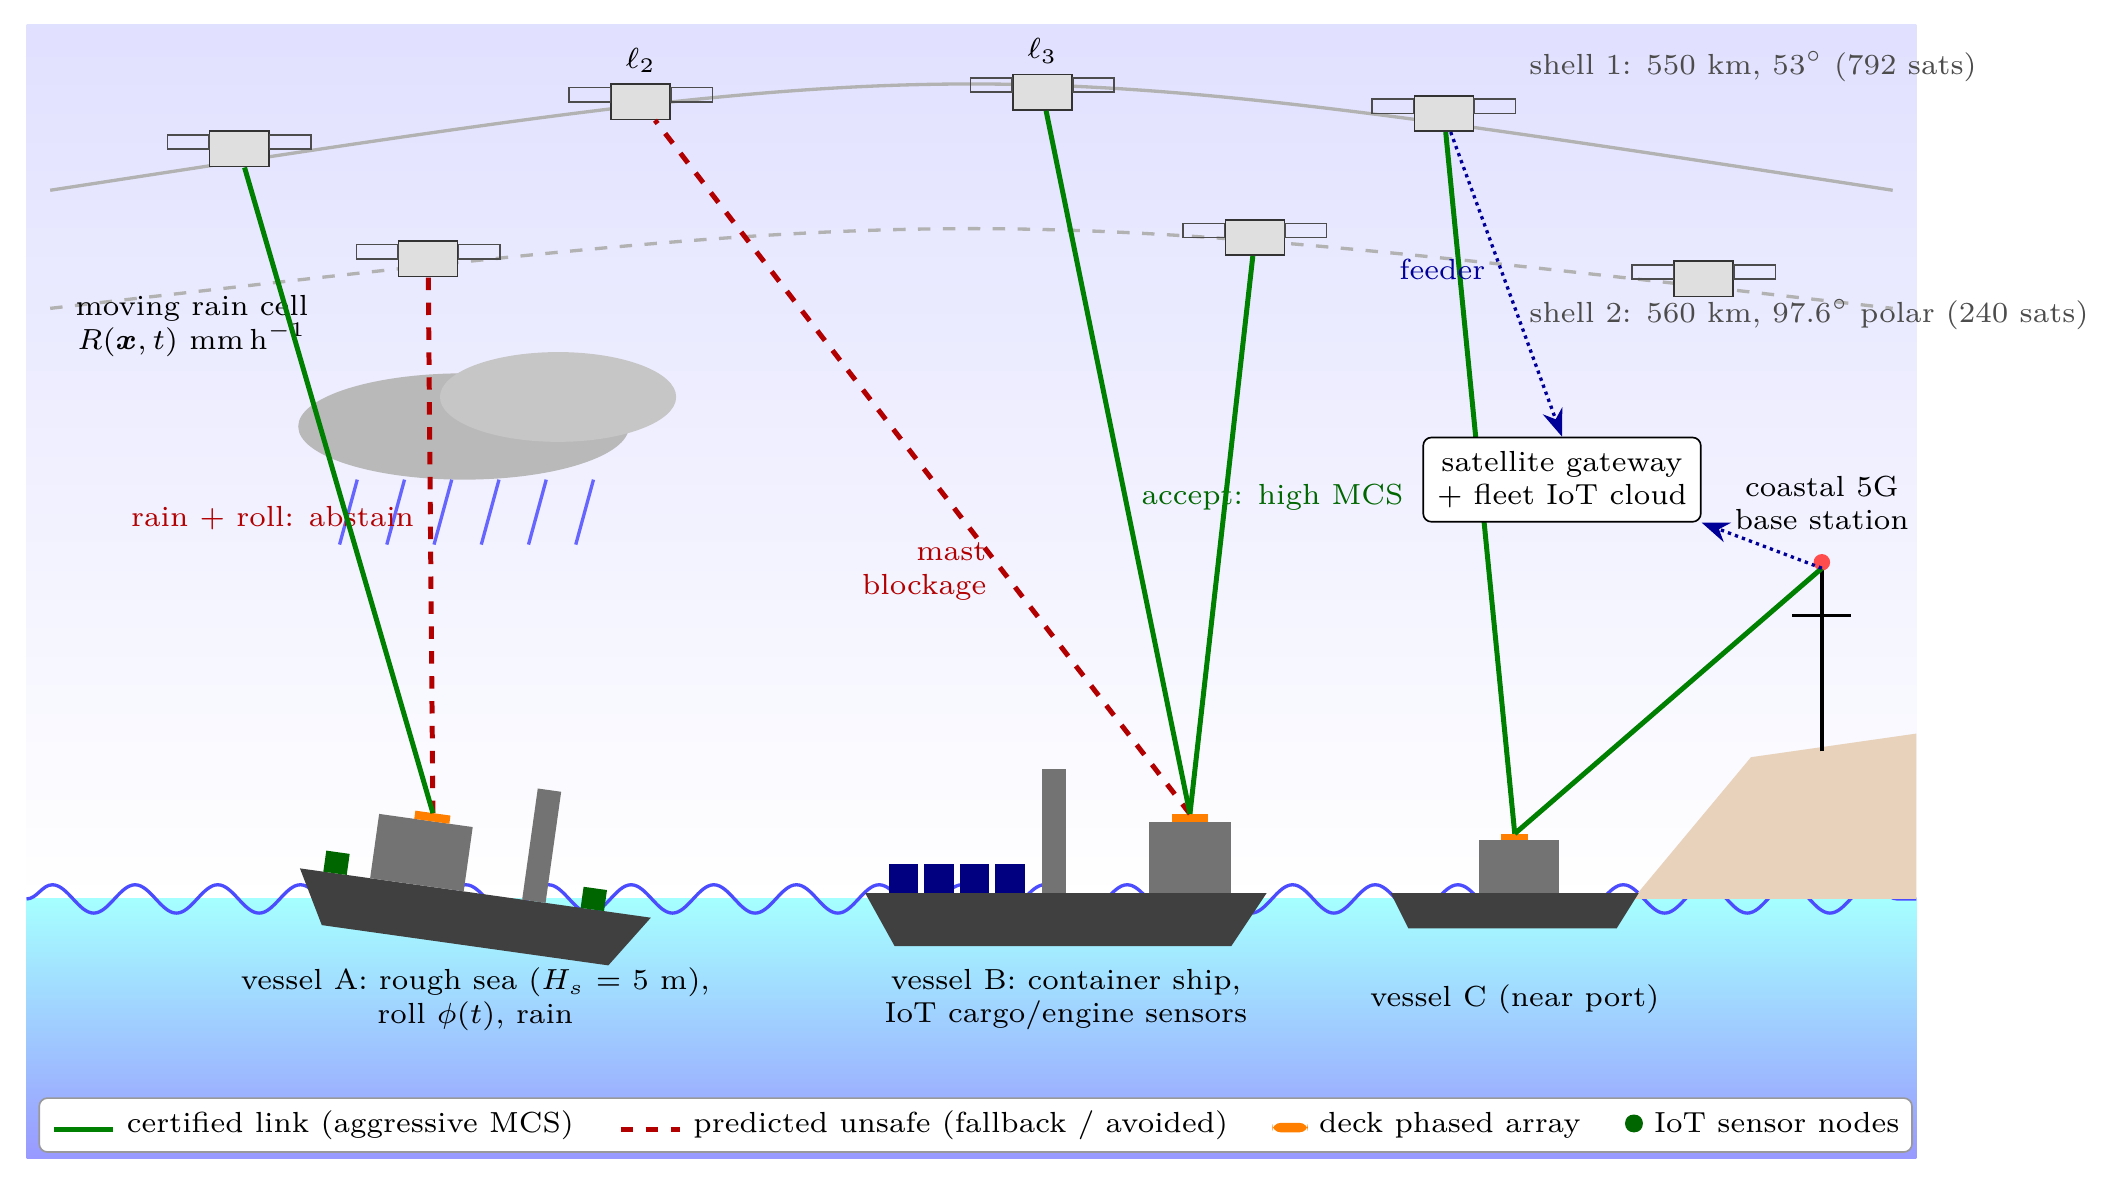
\includegraphics[width=\textwidth]{../figures/diagrams/sys_physical.png}
\caption{\textbf{Physical view of the maritime IoT satellite system.} Vessels select among visible LEO satellites of two shells and a coastal fifth-generation base station. Rain cells, ship roll and mast blockage make some links unsafe; certified links are used with an aggressive modulation and coding scheme, and unsafe decisions trigger the robust fallback.}
\label{fig:physical}
\end{figure}

\begin{figure}[t]
\centering
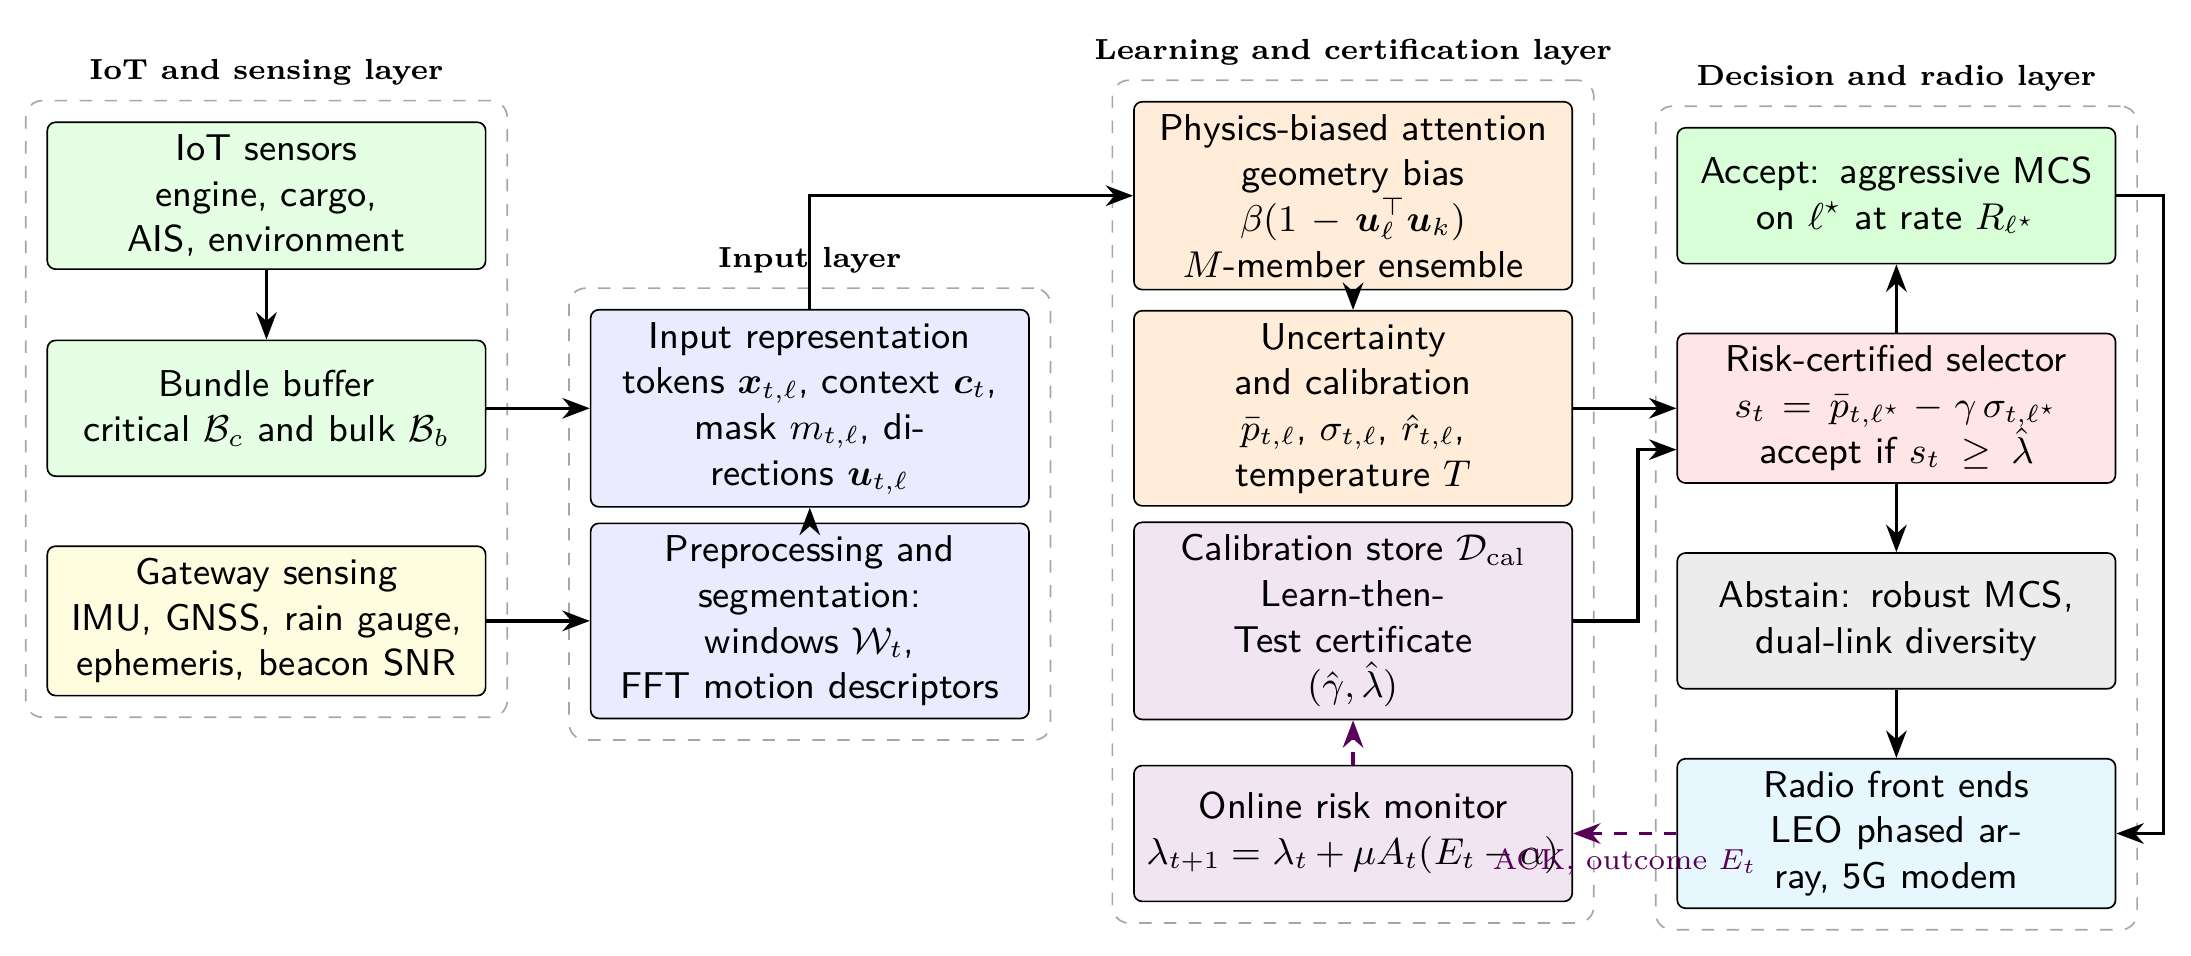
\includegraphics[width=\textwidth]{../figures/diagrams/sys_functional.png}
\caption{\textbf{Functional view of the SeaSel gateway.} Sensing data are segmented and tokenised, a physics-biased attention ensemble estimates link-success probabilities and their uncertainty, and a risk-certified selector either accepts an aggressive transmission or abstains to a robust dual-link mode. Outcomes feed the calibration store and the online risk monitor.}
\label{fig:functional}
\end{figure}

\begin{figure}[t]
\centering
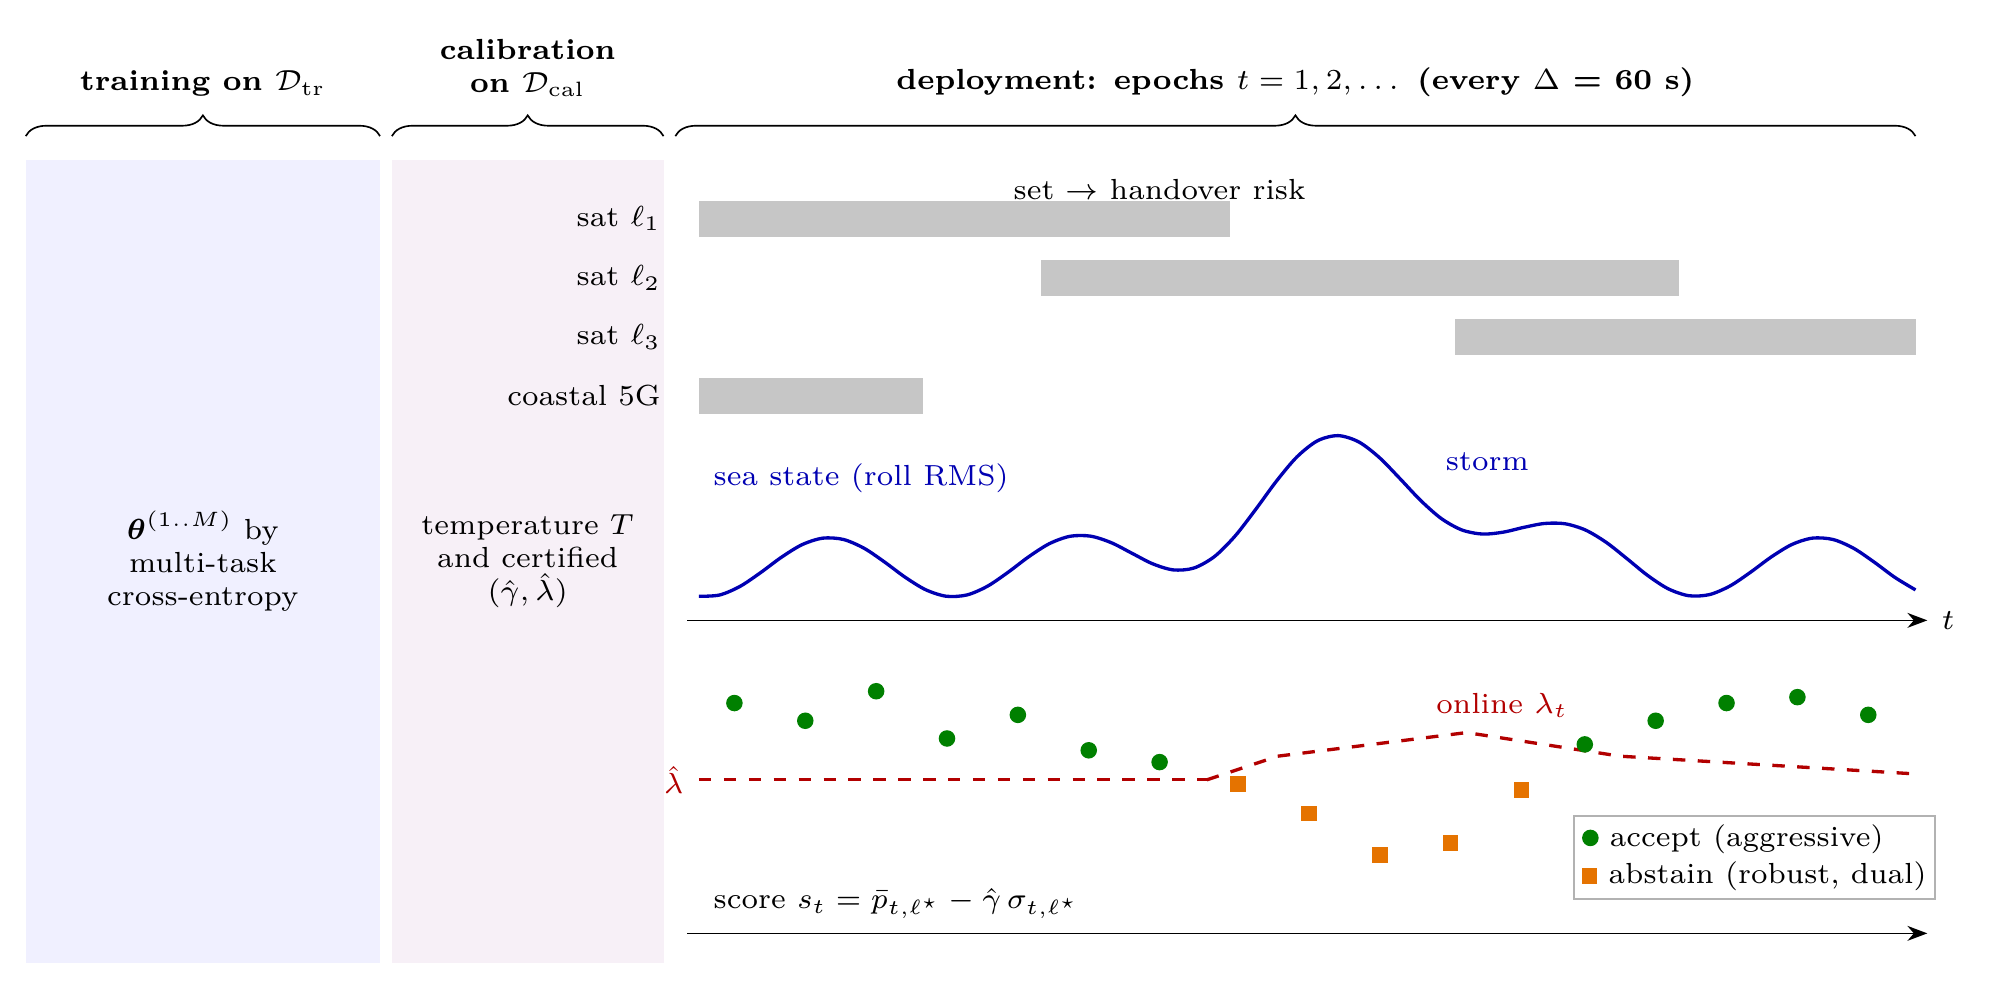
\includegraphics[width=\textwidth]{../figures/diagrams/sys_temporal.png}
\caption{\textbf{Temporal view of training, calibration and deployment.} During deployment the certified score $s_t$ is compared with the threshold $\hat\lambda$; when a storm degrades link quality, scores fall below the threshold and the gateway abstains, while the online monitor raises $\lambda_t$ if accepted decisions start to fail.}
\label{fig:temporal}
\end{figure}

Time is divided into decision epochs of duration $\Delta$. At epoch $t$, the gateway of vessel $v$ sees a candidate set $\mathcal L_t$ of at most $K$ satellites above the minimum elevation $\theta_{\min}$ plus, when within range, one coastal link. For a satellite link $\ell$ at range $d_{t,\ell}$ and elevation $\theta_{t,\ell}$, the signal-to-noise ratio of a transmission of duration $T_x$ is modelled as
\begin{equation}\label{eq:snr}
\mathrm{SNR}_{t,\ell}=\mathrm{SNR}_{\rm ref}-20\log_{10}\frac{d_{t,\ell}}{h_{\rm s}}-L^{\rm atm}_{t,\ell}-L^{\rm scan}_{t,\ell}-L^{\rm pt}_{t,\ell}-L^{\rm rain}_{t,\ell}-L^{\rm blk}_{t,\ell}+10\log_{10}|g_{t,\ell}|^{2}+\xi_{t,\ell},
\end{equation}
where $h_{\rm s}$ is the shell altitude, $g_{t,\ell}$ a Rician fading coefficient whose $K$-factor grows with elevation and $\xi_{t,\ell}$ scintillation. The deck normal $\bm n(\phi,\vartheta)$ rotates with roll $\phi$ and pitch $\vartheta$, so the scan angle of the array and the resulting scan loss are
\begin{equation}\label{eq:scan}
\cos\chi_{t,\ell}(\tau)=\bm n\big(\phi(\tau),\vartheta(\tau)\big)^{\top}\bm u^{\rm b}_{t,\ell},\qquad
L^{\rm scan}_{t,\ell}=-\frac{10\,n_{\rm s}}{T_x}\int_{t\Delta}^{t\Delta+T_x}\log_{10}\cos\chi_{t,\ell}(\tau)\,d\tau,
\end{equation}
with $\bm u^{\rm b}_{t,\ell}$ the satellite direction in the ship body frame and $n_{\rm s}$ the scan exponent. Motion also causes a tracking lag proportional to the angular rate $\omega_t$, giving the pointing loss
\begin{equation}\label{eq:pointing}
L^{\rm pt}_{t,\ell}=12\left(\frac{\kappa\,\omega_t}{\theta_{3\mathrm{dB}}}\right)^{2},
\end{equation}
where $\kappa$ is the tracking latency and $\theta_{3\mathrm{dB}}$ the beamwidth. Rain of rate $R_t$ attenuates the slant path through the rain layer of height $h_R$:
\begin{equation}\label{eq:rain}
L^{\rm rain}_{t,\ell}=a R_t^{\,b}\,\frac{L_s}{1+L_s\cos\theta_{t,\ell}/L_0},\qquad L_s=\frac{h_R}{\sin\theta_{t,\ell}}.
\end{equation}
A transmission succeeds in the aggressive mode, with rate $R_\ell$, or in the robust mode, with rate $R_0\ll R_\ell$, when
\begin{equation}\label{eq:labels}
Y_{t,\ell}=\mathbb 1\{\mathrm{SNR}_{t,\ell}\ge\eta_A\}\,\mathbb 1\{\theta_{t,\ell}(t\Delta+T_x)\ge\theta_{\min}\},\qquad
Y^{R}_{t,\ell}=\mathbb 1\{\mathrm{SNR}_{t,\ell}\ge\eta_R\}\,\mathbb 1\{\theta_{t,\ell}(t\Delta+T_x)\ge\theta_{\min}\},
\end{equation}
where the second factor captures handover failure when the satellite sets during the transmission.

\subsection{Traffic, transmission and feedback model}
Each vessel generates two traffic classes. A critical bundle $\mathcal B_c$ of a few kilobytes (alarms, safety telemetry, compliance reports) must be delivered within the epoch in which it is created; a bulk bundle $\mathcal B_b$ (engine logs, cargo telemetry, environmental sensor streams) is delay tolerant and benefits from every additional megabit. In each epoch the gateway makes a single transmission decision of duration $T_x$. In the aggressive mode it sends both bundles over one link with a high-order modulation and coding scheme; in the robust mode it sends the critical bundle, and as much bulk data as the low rate allows, over the two most reliable links with a low-order scheme, which doubles the radiated energy. Satellites and the coastal base station acknowledge every transmission, so the outcome $E_t$ of an accepted decision is known at the end of the epoch. This feedback is what makes the online rule of Section~\ref{sec:uq} possible. The gateway knows the ephemeris of every satellite, its own position and heading, its inertial measurements and the beacon SNR of the satellites it tracked in the previous epoch; it does not know the instantaneous rain field, the fading state or the exact roll during the transmission. Two assumptions underpin the guarantees: calibration and deployment epochs are exchangeable unless stated otherwise, and acknowledgements are reliable, which is reasonable because they are short and can be sent with the most robust scheme.

\subsection{Selective decision model}
Let $\bar p_{t,\ell}$ be the predicted aggressive-success probability, $\sigma_{t,\ell}$ its epistemic uncertainty and $\hat r_{t,\ell}$ the predicted robust-success probability. The gateway chooses the link with the highest expected aggressive goodput and forms an uncertainty-penalised confidence score:
\begin{equation}\label{eq:choice}
\ell^\star_t=\arg\max_{\ell\in\mathcal L_t}\ \bar p_{t,\ell}R_\ell,\qquad
s_t(\gamma)=\bar p_{t,\ell^\star_t}-\gamma\,\sigma_{t,\ell^\star_t},
\end{equation}
and accepts the aggressive transmission only when the score clears a threshold:
\begin{equation}\label{eq:accept}
A_t(\gamma,\lambda)=\mathbb 1\{s_t(\gamma)\ge\lambda\}.
\end{equation}
When $A_t=0$ the gateway abstains and sends the critical bundle in the robust mode duplicated over the two links with the highest $\hat r_{t,\ell}$, which costs twice the energy. Writing $E_t=1-Y_{t,\ell^\star_t}$ for an aggressive failure and $F_t$ for a failure of the robust fallback, the selective risk, the critical-message miss rate and the goodput are
\begin{equation}\label{eq:selrisk}
R_{\rm sel}(\gamma,\lambda)=\Pr\big[E_t=1\mid A_t(\gamma,\lambda)=1\big],
\end{equation}
\begin{equation}\label{eq:miss}
\mathcal M(\gamma,\lambda)=\Pr[A_t=1,E_t=1]+\Pr[A_t=0,F_t=1],
\end{equation}
\begin{equation}\label{eq:goodput}
\mathcal G(\gamma,\lambda)=T_x\,\mathbb E\big[A_t(1-E_t)R_{\ell^\star_t}+(1-A_t)(1-F_t)R_0\big].
\end{equation}

\subsection{Risk-constrained objective}
The design problem is to maximise goodput while guaranteeing that accepted aggressive transmissions fail rarely:
\begin{equation}\label{eq:objective}
\max_{\gamma,\lambda}\ \mathcal G(\gamma,\lambda)\quad\text{subject to}\quad \Pr_{\mathcal D_{\rm cal}}\big[R_{\rm sel}(\hat\gamma,\hat\lambda)\le\alpha\big]\ge1-\delta,
\end{equation}
where the probability is over the random calibration set $\mathcal D_{\rm cal}$, $\alpha$ is the tolerated selective risk and $\delta$ the confidence parameter. Because the coverage $c=\Pr[A_t=1]$ and the fallback failure probability $\rho_F=\Pr[F_t=1\mid A_t=0]$ are measurable, constraint (\ref{eq:objective}) bounds the miss rate directly:
\begin{equation}\label{eq:missbound}
\mathcal M\le c\,\alpha+(1-c)\,\rho_F .
\end{equation}

\subsection{Motivation for selective prediction}
Two naive designs bracket the problem. Always transmitting aggressively maximises goodput but lets every prediction error become a lost critical message. Always transmitting robustly protects critical messages but reduces goodput by an order of magnitude and doubles energy per bit. Tuning a confidence threshold on validation data sits in between, but its risk is uncontrolled: the threshold is a point estimate and can exceed the target on new data, as the experiments confirm. Selective prediction with certification resolves this tension. The predictor acts where it is reliable, abstains where it is not, and the certificate (\ref{eq:objective}) turns the abstention threshold into an engineering parameter with a guaranteed meaning. Through bound (\ref{eq:missbound}) it also converts a statistical guarantee into a service-level guarantee for maritime IoT. As an illustration, with $\alpha=0.05$, a coverage of 90\% and a fallback failure probability of 2\%, the bound gives a miss rate of at most 4.7\%, while the vessel still uses the aggressive scheme in nine epochs out of ten.

\begin{table}[t]
\centering\small
\caption{\textbf{Symbols and notation.}}
\label{tab:symbols}
\begin{tabular}{@{}ll@{\hspace{1.2em}}ll@{}}
\toprule
Symbol & Meaning & Symbol & Meaning\\\midrule
$\mathcal V$, $v$ & vessels, vessel index & $t$, $\Delta$ & decision epoch, epoch duration\\
$\mathcal L_t$, $\ell$, $K$ & candidate links, link, max.\ satellites & $T_x$ & transmission duration\\
$\theta_{t,\ell}$, $d_{t,\ell}$ & elevation, slant range & $\bm u_{t,\ell}$ & unit direction to link $\ell$\\
$\phi$, $\vartheta$, $\omega_t$ & roll, pitch, angular rate & $H_s$ & significant wave height\\
$\chi_{t,\ell}$, $n_{\rm s}$ & scan angle, scan exponent & $\kappa$, $\theta_{3\mathrm{dB}}$ & tracking latency, beamwidth\\
$R_t$, $h_R$ & rain rate, rain height & $a$, $b$ & rain attenuation coefficients\\
$\eta_A$, $\eta_R$ & aggressive / robust SNR thresholds & $R_\ell$, $R_0$ & aggressive / robust rates\\
$Y_{t,\ell}$, $Y^R_{t,\ell}$ & aggressive / robust success & $\bm x_{t,\ell}$, $\bm c_t$ & link token, vessel context\\
$m_{t,\ell}$ & validity mask & $\mathcal W_t$ & IMU segment for epoch $t$\\
$\bar p_{t,\ell}$, $\sigma_{t,\ell}$ & ensemble mean, spread & $\hat r_{t,\ell}$ & robust-success probability\\
$M$, $T$ & ensemble size, temperature & $\beta$ & physics-bias strength\\
$s_t$, $\gamma$, $\lambda$ & score, uncertainty penalty, threshold & $A_t$, $E_t$, $F_t$ & accept, aggressive / fallback failure\\
$R_{\rm sel}$, $c$ & selective risk, coverage & $\mathcal M$, $\mathcal G$ & miss rate, goodput\\
$\alpha$, $\delta$ & target risk, confidence & $\mathcal D_{\rm tr}$, $\mathcal D_{\rm cal}$ & training and calibration sets\\
$\mu$ & online step size & $g(\cdot)$ & sea-state group\\
\bottomrule
\end{tabular}
\end{table}

% ===========================================================================
\section{New algorithm: SeaSel}\label{sec:algo}
% ===========================================================================
Algorithm~1 summarises SeaSel. It has three phases. In the offline phase, an ensemble of physics-biased attention networks is trained on logged epochs $\mathcal D_{\rm tr}$ with a multi-task loss that predicts aggressive and robust success (Section~\ref{sec:arch}), and a temperature is fitted on a validation split. In the calibration phase, a held-out set $\mathcal D_{\rm cal}$ of $n$ epochs is used to certify a pair $(\hat\gamma,\hat\lambda)$ by Learn-then-Test (Section~\ref{sec:uq}). In the deployment phase, the gateway evaluates the ensemble once per epoch, applies the certified rule (\ref{eq:accept}), transmits and, when acknowledgements reveal drift, updates the threshold online.

\begin{center}
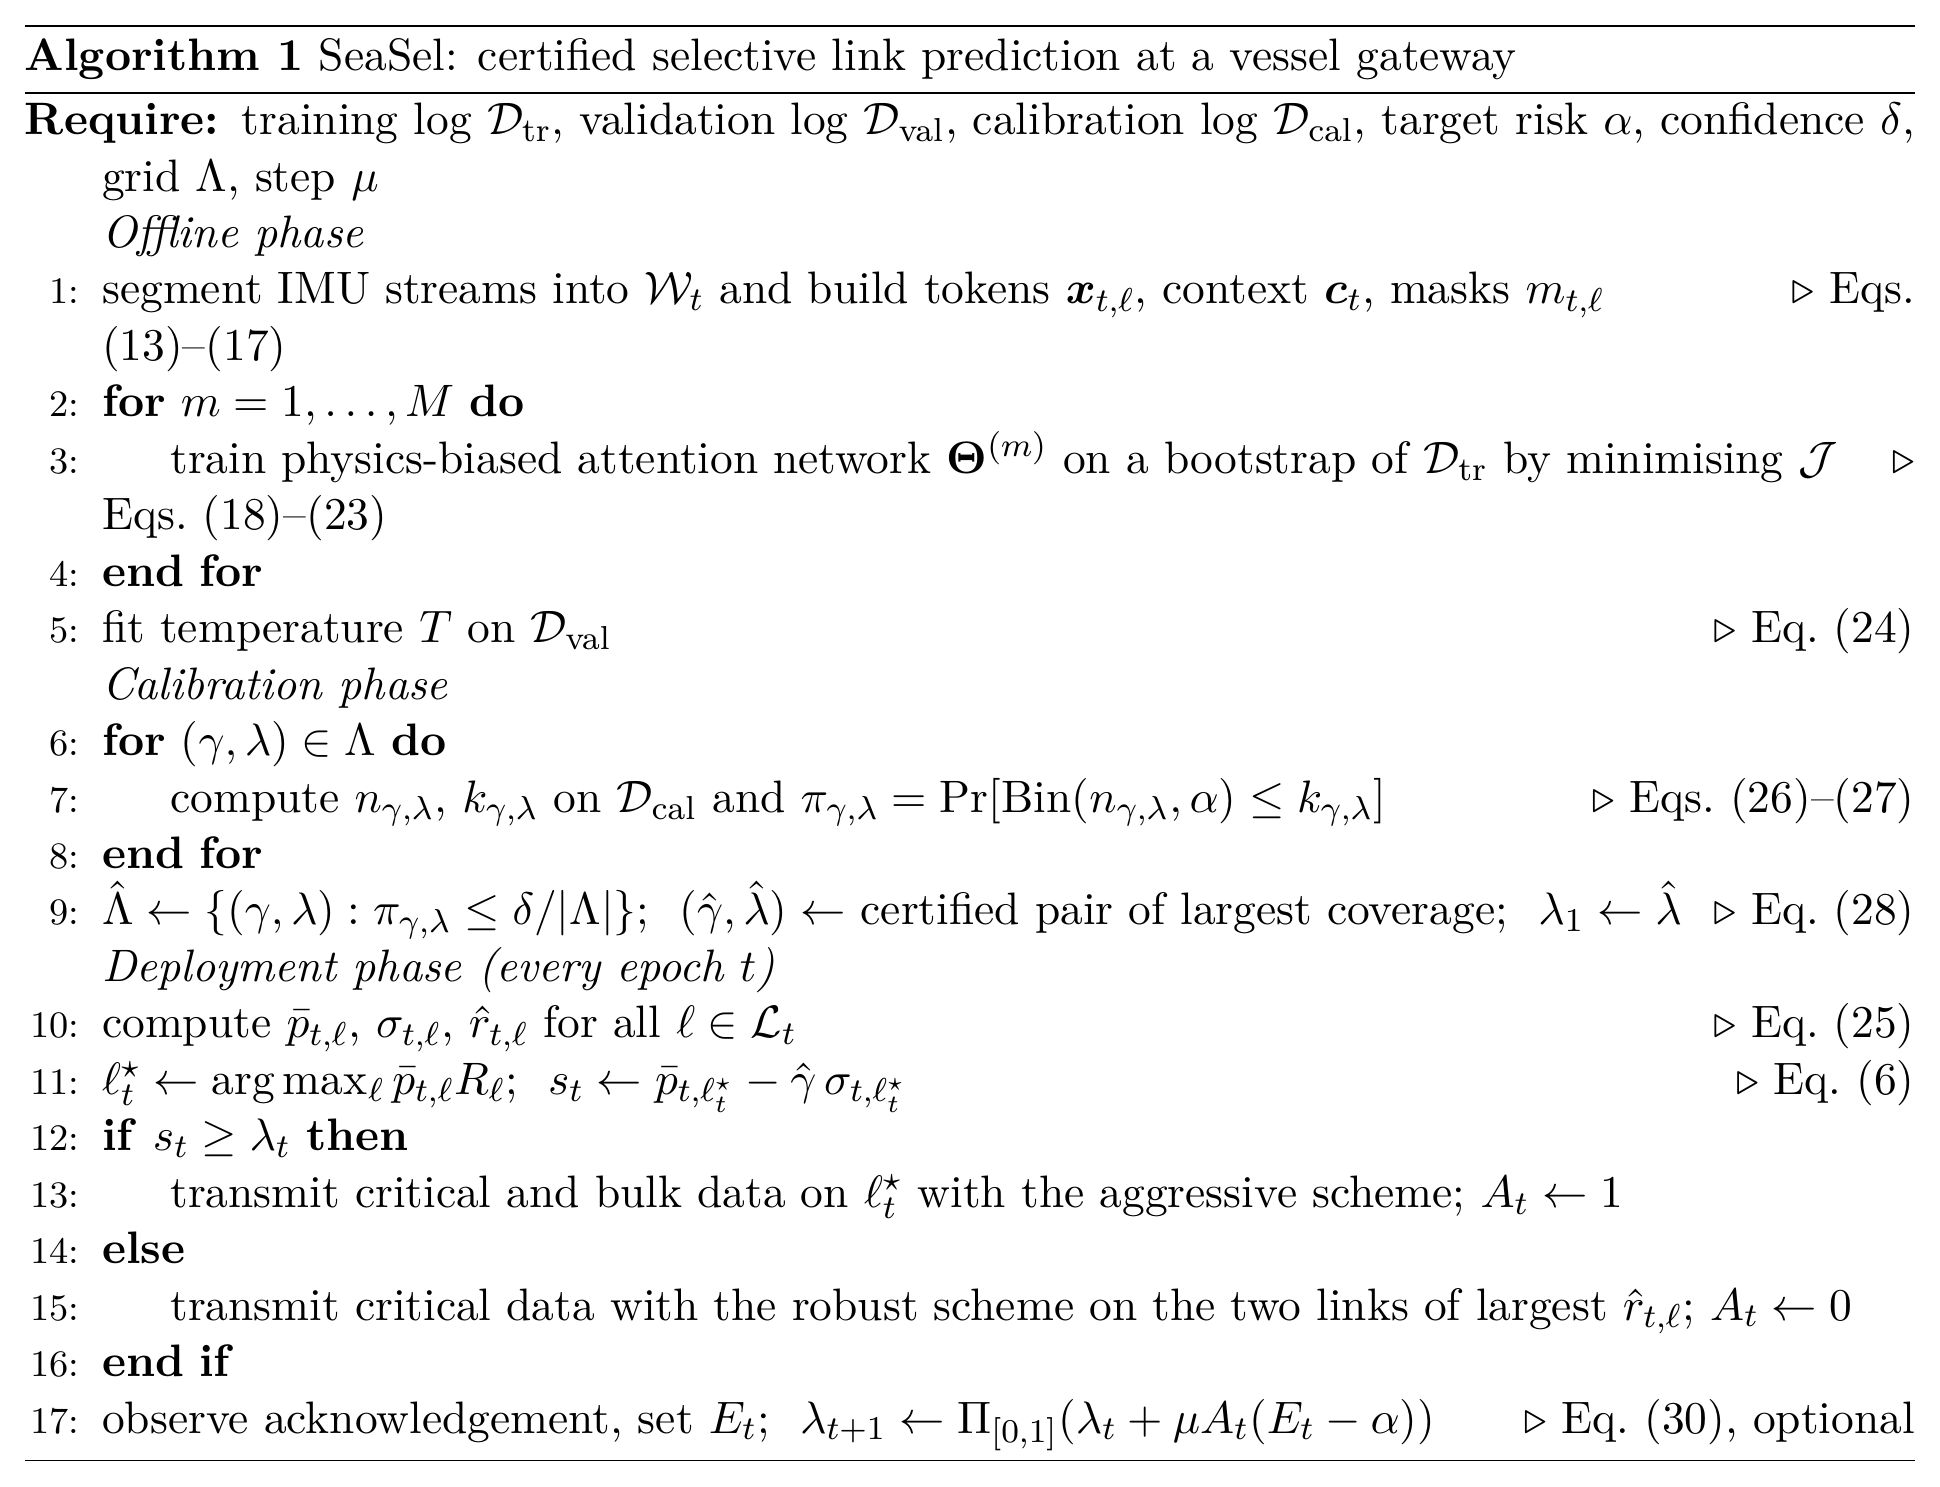
\includegraphics[width=0.97\textwidth]{../figures/diagrams/algorithm.png}
\end{center}

The certification step rests on the following result.

\begin{theorem}[Certified selective risk]\label{thm:cert}
Let the calibration epochs and a test epoch be independent and identically distributed, and let $\Lambda$ be a finite grid of $(\gamma,\lambda)$ pairs. For each pair, let $n_{\gamma,\lambda}$ be the number of accepted calibration epochs and $k_{\gamma,\lambda}$ the number of aggressive failures among them. Define the p-value $\pi_{\gamma,\lambda}=\Pr[\mathrm{Bin}(n_{\gamma,\lambda},\alpha)\le k_{\gamma,\lambda}]$ and the certified set $\hat\Lambda=\{(\gamma,\lambda)\in\Lambda:\pi_{\gamma,\lambda}\le\delta/|\Lambda|\}$. Then any pair selected from $\hat\Lambda$, in particular the one maximising calibration coverage, satisfies $\Pr[R_{\rm sel}(\hat\gamma,\hat\lambda)\le\alpha]\ge1-\delta$.
\end{theorem}
\noindent\textit{Proof.} Fix $(\gamma,\lambda)$ with $R_{\rm sel}(\gamma,\lambda)>\alpha$. Conditionally on $n_{\gamma,\lambda}$, the accepted calibration epochs are independent draws from the distribution conditioned on $\{s_t(\gamma)\ge\lambda\}$, so $k_{\gamma,\lambda}\sim\mathrm{Bin}(n_{\gamma,\lambda},R_{\rm sel})$, which stochastically dominates $\mathrm{Bin}(n_{\gamma,\lambda},\alpha)$. Hence $\Pr[\pi_{\gamma,\lambda}\le u]\le u$ for all $u$, so $\pi_{\gamma,\lambda}$ is a valid p-value. By the union bound over the at most $|\Lambda|$ pairs whose null hypothesis is true, the probability that any of them enters $\hat\Lambda$ is at most $\delta$. On the complementary event every certified pair has $R_{\rm sel}\le\alpha$, whatever rule is then used to choose among them\cite{angelopoulos2025,bates2021}. $\square$

\begin{proposition}[Service-level guarantee]\label{prop:service}
On the event of Theorem~\ref{thm:cert}, the critical-message miss rate obeys (\ref{eq:missbound}). If, in addition, the fallback failure probability satisfies $\rho_F\le\rho$, then $\mathcal M\le\alpha c+\rho(1-c)\le\max(\alpha,\rho)$, and the goodput satisfies $\mathcal G\ge T_x\big[c(1-\alpha)\min_\ell R_\ell+(1-c)(1-\rho)R_0\big]$.
\end{proposition}
\noindent\textit{Proof.} Equation~(\ref{eq:miss}) gives $\mathcal M=c\,R_{\rm sel}+(1-c)\rho_F$; substituting $R_{\rm sel}\le\alpha$ and $\rho_F\le\rho$ yields both inequalities. Equation~(\ref{eq:goodput}) is bounded in the same way term by term. $\square$

The calibration cost is $O(|\Lambda|\,n)$ and is performed once per calibration window. The deployment cost per epoch is one forward pass of $M$ small networks over at most $K+1$ tokens, which is dominated by the attention product and scales as $O(M K^2 d)$, with $d$ the model width.

% ===========================================================================
\section{Preprocessing, segmentation, and input representation}\label{sec:prep}
% ===========================================================================
\textbf{Segmentation.} The inertial measurement unit samples roll $\phi$ and pitch $\vartheta$ at $f_s=2$\,Hz. For epoch $t$ the gateway extracts the segment immediately preceding the decision,
\begin{equation}\label{eq:segment}
\mathcal W_t=\big\{(\phi(\tau),\vartheta(\tau)):\ t\Delta-w\le\tau<t\Delta\big\},\qquad w=60\ {\rm s},
\end{equation}
so no information from the transmission itself leaks into the input. Each segment is summarised by root-mean-square motion and angular rate,
\begin{equation}\label{eq:rms}
\bar\phi_t=\Big(\tfrac1{|\mathcal W_t|}\textstyle\sum_{\mathcal W_t}\phi^2\Big)^{1/2},\quad
\bar\vartheta_t=\Big(\tfrac1{|\mathcal W_t|}\textstyle\sum_{\mathcal W_t}\vartheta^2\Big)^{1/2},\quad
\omega_t=f_s\Big(\tfrac1{|\mathcal W_t|}\textstyle\sum_{\mathcal W_t}(\Delta\phi)^2+(\Delta\vartheta)^2\Big)^{1/2},
\end{equation}
and by the dominant motion period obtained from the periodogram of the roll signal:
\begin{equation}\label{eq:period}
P_t=\Big(\arg\max_{f>0}\left|\textstyle\sum_{\tau\in\mathcal W_t}(\phi(\tau)-\bar\phi^{\rm m}_t)e^{-j2\pi f\tau}\right|^2\Big)^{-1},
\end{equation}
where $\bar\phi^{\rm m}_t$ is the segment mean. The rain-gauge reading is log-compressed, $\tilde R_t=\log(1+R_t)+\epsilon_t$ with sensor noise $\epsilon_t$.

\textbf{Input representation.} The vessel context is $\bm c_t=[\bar\phi_t,\bar\vartheta_t,\omega_t,P_t,\tilde R_t,v_t,\log(1+d^{\rm port}_t)]$, where $v_t$ is the ship speed and $d^{\rm port}_t$ the distance to the nearest port. Each candidate link becomes a token
\begin{equation}\label{eq:token}
\bm x_{t,\ell}=\Big[\tfrac{\theta_{t,\ell}}{90},\sin\psi^{\rm r}_{t,\ell},\cos\psi^{\rm r}_{t,\ell},\dot\theta_{t,\ell},\log(1+\tau^{\rm set}_{t,\ell}),\tfrac{\chi^0_{t,\ell}}{90},e^{\rm sec}_{t,\ell},\tfrac{\Delta^{\rm b}_{t-1,\ell}}{10},h_{t,\ell},\iota_{t,\ell},\log(1+d_{t,\ell}),\tfrac{\mathrm{SNR}^{\rm cs}_{t,\ell}}{10}\Big],
\end{equation}
containing the elevation, the azimuth $\psi^{\rm r}$ relative to the heading, the elevation rate, the time to setting from the ephemeris, the scan angle on a level deck, an exponentially weighted blockage evidence for the azimuth sector, the last observed beacon deficit $\Delta^{\rm b}$ (clear-sky prediction minus measured beacon SNR) with its availability flag $h$, a coastal-link indicator $\iota$, the range and the clear-sky SNR. The unit direction $\bm u_{t,\ell}$ is kept separately for the attention bias. Up to $K=8$ satellites ordered by elevation and one coastal token form a padded set with mask $m_{t,\ell}\in\{0,1\}$.

\textbf{Normalisation.} With mean $\mu_j$ and standard deviation $s_j$ of feature $j$ computed over valid training tokens only, every feature is standardised and masked:
\begin{equation}\label{eq:norm}
\tilde x_{t,\ell,j}=m_{t,\ell}\,\frac{x_{t,\ell,j}-\mu_j}{s_j},
\end{equation}
and missing values (sensor dropouts) are set to the training mean, i.e.\ zero after standardisation. Training, validation and calibration splits are formed by vessel, so that no vessel contributes to both training and evaluation.

% ===========================================================================
\section{Proposed attention-enhanced maritime IoT satellite architecture}\label{sec:arch}
% ===========================================================================
Each token is first embedded together with the vessel context,
\begin{equation}\label{eq:embed}
\bm h^{0}_{t,\ell}=\mathrm{ReLU}\big(\bm W_1[\tilde{\bm x}_{t,\ell};\tilde{\bm c}_t]+\bm b_1\big)\in\mathbb R^{d}.
\end{equation}
The key element is a self-attention layer over the candidate set whose logits contain a geometric prior. Links that point to nearby directions share rain cells, blockage sectors and motion-induced scan loss, so the attention logit between links $\ell$ and $k$ is
\begin{equation}\label{eq:pba}
e_{\ell k}=\frac{(\bm W_q\bm h^0_{t,\ell})^{\top}(\bm W_k\bm h^0_{t,k})}{\sqrt{d_k}}-\operatorname{softplus}(\beta)\big(1-\bm u_{t,\ell}^{\top}\bm u_{t,k}\big)+\log m_{t,k},
\end{equation}
where $\beta$ is learned and $\log m_{t,k}=-\infty$ removes padded tokens. The attention weights and the updated representation are
\begin{equation}\label{eq:softmax}
a_{\ell k}=\frac{\exp e_{\ell k}}{\sum_{k'}\exp e_{\ell k'}},\qquad
\bm h^{1}_{t,\ell}=\bm h^{0}_{t,\ell}+\bm W_o\sum_k a_{\ell k}\bm W_v\bm h^{0}_{t,k},
\end{equation}
followed by a residual feed-forward block
\begin{equation}\label{eq:ffn}
\bm h^{2}_{t,\ell}=\bm h^{1}_{t,\ell}+\bm W_3\,\mathrm{ReLU}\big(\bm W_2\bm h^{1}_{t,\ell}+\bm b_2\big).
\end{equation}
Because (\ref{eq:pba})--(\ref{eq:ffn}) act on sets, the network is permutation equivariant and handles any number of visible satellites. The bias term is new: with $\beta\to-\infty$ it reduces to standard attention, while large $\beta$ restricts communication to geometrically close links. Two heads produce logits for aggressive and robust success,
\begin{equation}\label{eq:heads}
\big[z^{A}_{t,\ell},\ z^{R}_{t,\ell}\big]=\bm W_{\rm out}^{\top}\bm h^{2}_{t,\ell}+\bm b_{\rm out},
\end{equation}
trained jointly by the masked multi-task cross-entropy
\begin{equation}\label{eq:loss}
\mathcal J(\bm\Theta)=\frac{\sum_{t,\ell}m_{t,\ell}\big[\mathrm{BCE}(z^A_{t,\ell},Y_{t,\ell})+\mathrm{BCE}(z^R_{t,\ell},Y^R_{t,\ell})\big]}{\sum_{t,\ell}m_{t,\ell}}+\lambda_2\sum_j\|\bm W_j\|_F^2,
\end{equation}
with $\mathrm{BCE}(z,y)=\log(1+e^{z})-yz$ and weight decay $\lambda_2$. The model has width $d=32$, key dimension $d_k=16$ and \RParams{} parameters per member, small enough for an embedded gateway processor. Each of the $M=5$ ensemble members is trained on a bootstrap resample of $\mathcal D_{\rm tr}$ with a different initialisation, using Adam with a cosine learning-rate schedule for 12 epochs.

% ===========================================================================
\section{Uncertainty estimation, calibration, and risk-controlled selective prediction}\label{sec:uq}
% ===========================================================================
\textbf{Ensemble uncertainty and temperature scaling.} With member logits $z^{A,(m)}_{t,\ell}$ and a temperature $T$ fitted by minimising the validation negative log-likelihood,
\begin{equation}\label{eq:temp}
T=\arg\min_{T>0}\ -\!\!\sum_{(t,\ell)\in\mathcal D_{\rm val}}\!\!\Big[Y_{t,\ell}\log\varsigma\Big(\tfrac{\bar z_{t,\ell}}{T}\Big)+(1-Y_{t,\ell})\log\Big(1-\varsigma\Big(\tfrac{\bar z_{t,\ell}}{T}\Big)\Big)\Big],
\end{equation}
where $\varsigma$ is the logistic function and $\bar z$ the ensemble-mean logit, the calibrated probability and the epistemic spread are
\begin{equation}\label{eq:ensemble}
\bar p_{t,\ell}=\frac1M\sum_{m=1}^{M}\varsigma\Big(\tfrac{z^{A,(m)}_{t,\ell}}{T}\Big),\qquad
\sigma_{t,\ell}=\Big(\frac1M\sum_{m=1}^{M}\Big[\varsigma\Big(\tfrac{z^{A,(m)}_{t,\ell}}{T}\Big)-\bar p_{t,\ell}\Big]^2\Big)^{1/2}.
\end{equation}
The robust-success probability $\hat r_{t,\ell}$ is obtained in the same way from $z^R$ and selects the two fallback links.

\textbf{Risk-controlled selective prediction.} For every pair on the grid $\Lambda=\{0,0.5,1,2\}\times\{0.30,\dots,0.99\}$ ($4\times70$ pairs), the gateway counts accepted calibration epochs and their failures,
\begin{equation}\label{eq:counts}
n_{\gamma,\lambda}=\sum_{i\in\mathcal D_{\rm cal}}A_i(\gamma,\lambda),\qquad k_{\gamma,\lambda}=\sum_{i\in\mathcal D_{\rm cal}}A_i(\gamma,\lambda)E_i,
\end{equation}
computes the exact binomial p-value
\begin{equation}\label{eq:pvalue}
\pi_{\gamma,\lambda}=\sum_{j=0}^{k_{\gamma,\lambda}}\binom{n_{\gamma,\lambda}}{j}\alpha^{j}(1-\alpha)^{n_{\gamma,\lambda}-j},
\end{equation}
and selects, among the pairs certified by Theorem~\ref{thm:cert}, the one with the largest calibration coverage:
\begin{equation}\label{eq:select}
(\hat\gamma,\hat\lambda)=\arg\max_{(\gamma,\lambda)\in\hat\Lambda}\ \frac{n_{\gamma,\lambda}}{|\mathcal D_{\rm cal}|},\qquad \hat\Lambda=\Big\{(\gamma,\lambda):\pi_{\gamma,\lambda}\le\frac{\delta}{|\Lambda|}\Big\}.
\end{equation}
If $\hat\Lambda$ is empty the gateway always abstains, which is safe by construction.

\textbf{Sea-state-conditional certification.} A pooled certificate controls risk on average over sea states. Storms concentrate failures in rough conditions, so SeaSel can certify separately within sea-state groups $g(\bar\phi_t)\in\{\text{calm},\text{moderate},\text{rough}\}$ defined by roll-RMS terciles,
\begin{equation}\label{eq:mondrian}
(\hat\gamma_g,\hat\lambda_g)=\arg\max_{(\gamma,\lambda)\in\hat\Lambda_g}\ \frac{n^{(g)}_{\gamma,\lambda}}{|\mathcal D^{(g)}_{\rm cal}|},
\end{equation}
which gives the guarantee of Theorem~\ref{thm:cert} conditionally on each group.

\textbf{Online risk adaptation.} When the environment drifts beyond the calibration distribution, acknowledgements reveal $E_t$ for accepted epochs and the threshold is updated as
\begin{equation}\label{eq:online}
\lambda_{t+1}=\Pi_{[0,1]}\big(\lambda_t+\mu\,A_t(E_t-\alpha)\big),
\end{equation}
where $\Pi_{[0,1]}$ is projection and $\mu$ the step size. Summing (\ref{eq:online}) over a horizon $H$ during which the projection is inactive gives
\begin{equation}\label{eq:longrun}
\frac{1}{H}\sum_{t=1}^{H}A_t(E_t-\alpha)=\frac{\lambda_{H+1}-\lambda_1}{\mu H}\le\frac{1}{\mu H},
\end{equation}
so the long-run joint failure rate of accepted epochs converges to at most $\alpha$ times the long-run coverage, without any distributional assumption\cite{barber2023}. The pooled certificate, the conditional certificate and the online rule are compared under distribution shift in Section~\ref{sec:ablation}.

% ===========================================================================
\section{Baselines and experimental setup}\label{sec:setup}
% ===========================================================================
\subsection{Sandbox testbed}
All experiments run in an open, sandboxed digital testbed that generates every observation available to a vessel gateway together with the ground-truth outcome of transmitting on every candidate link (Table~\ref{tab:params}). The space segment consists of two Walker-delta shells, 792 satellites at 550\,km and 53$^\circ$ inclination and 240 polar satellites at 560\,km and 97.6$^\circ$, propagated with Earth rotation; this mirrors the layered shells of current broadband constellations\cite{kodheli2021,michel2022}. Forty vessels sail great-circle routes between twelve major ports at 10--22 knots, so the data include open-ocean, high-latitude and near-port segments. A sea-state field combines a latitude climate with storms that move across vessel tracks and carry both waves and rain; background convective rain cells add further variability. Roll and pitch are synthesised at 2\,Hz from a narrow-band wave spectrum centred on each vessel's natural period, with amplitude proportional to the local significant wave height. Each vessel has one or two superstructure blockage sectors. Link outcomes follow equations (\ref{eq:snr})--(\ref{eq:labels}) with Rician fading, scintillation and handover failure; coastal links follow a sea-path loss with a slowly varying ducting term near ports.

The training day (seed 0) provides 24 vessels for training, 4 for validation and 12 held-out vessels; an independent day (seed 1) provides 40 further vessels. The held-out vessels and the independent day form the evaluation pool of \RNPool{} epochs, which is split at random 100 times into equal calibration and test halves. Three shifted days test out-of-distribution behaviour: severe storms (significant wave height up to 9.5\,m against 6.4\,m in training, rain up to 88\,mm\,h$^{-1}$, storms on 85\% of tracks), tropical routes with frequent heavy convective rain, and a degraded constellation in which 30\% of satellites have failed and the remainder suffer a 2\,dB ageing loss. In the evaluation pool, an aggressive transmission on a random candidate succeeds with probability \RPAggr\%, a robust one with probability \RPRob\%, a vessel sees \RNCand{} candidates on average, and \RNoLink\% of epochs have no usable link at all.

\begin{table}[t]
\centering\small
\caption{\textbf{Testbed and training parameters.}}
\label{tab:params}
\begin{tabular}{@{}ll@{\hspace{1.5em}}ll@{}}
\toprule
Parameter & Value & Parameter & Value\\\midrule
Shell 1 & 550 km, 53$^\circ$, $36\times22$ & Shell 2 & 560 km, 97.6$^\circ$, $12\times20$\\
Minimum elevation $\theta_{\min}$ & 25$^\circ$ & Candidates $K$ & 8 satellites + 1 coastal\\
Epoch $\Delta$, transmission $T_x$ & 60 s, 20 s & Vessels per day, horizon & 40, 24 h\\
$\mathrm{SNR}_{\rm ref}$ (zenith) & 23 dB & Scan exponent $n_{\rm s}$, max scan & 1.3, 70$^\circ$\\
Beamwidth $\theta_{3\mathrm{dB}}$ & 3$^\circ$ & Blockage loss & 25 dB\\
Rain law $a$, $b$, $h_R$ & 0.0374, 1.15, 4 km & Thresholds $\eta_A$, $\eta_R$ & 10 dB, $-2$ dB\\
Rates $R_\ell$ (satellite, coastal), $R_0$ & 20, 40, 1 Mbit\,s$^{-1}$ & Transmit power & 10 W\\
IMU rate, segment $w$ & 2 Hz, 60 s & Model width $d$, $d_k$ & 32, 16\\
Ensemble $M$, epochs & 5, 12 & Optimiser & Adam, cosine, $3\times10^{-3}$\\
Target $\alpha$, confidence $\delta$ & 0.05, 0.10 & Grid $|\Lambda|$ & $4\times70$\\
Online step $\mu$ & 0.02 & Calibration/test splits & 100\\
\bottomrule
\end{tabular}
\end{table}

\subsection{Baselines}
Eight policies are compared, all using the same aggressive and robust transmission schemes. \emph{Max-elevation} always transmits aggressively on the highest satellite (or the coastal link when available), the classical rule for LEO terminals. \emph{Always robust} always uses the dual-link robust mode. \emph{Link-budget margin} predicts the SNR margin from the clear-sky budget and the last beacon deficit and accepts above a margin tuned on validation data. \emph{Logistic regression} and \emph{gradient boosting} are per-link classifiers on the same token and context features, with a softmax-response threshold tuned on validation data to reach $\alpha$ without certification\cite{hendrickx2024}. \emph{Gradient boosting with LTT} applies the SeaSel certificate to the gradient-boosting predictor, isolating the contribution of the model. \emph{PBA single model} applies the certificate to one physics-biased attention network without ensemble uncertainty. \emph{SeaSel} is the full method.

\subsection{Metrics and protocol}
Reported metrics are the coverage $c$, the selective risk $R_{\rm sel}$, the critical-message miss rate $\mathcal M$, the goodput $\mathcal G$, the energy per delivered megabit, the violation frequency (fraction of the 100 splits in which $R_{\rm sel}>\alpha$, which Theorem~\ref{thm:cert} bounds by $\delta$), the area under the receiver operating characteristic curve (AUROC), the expected calibration error (ECE) and the area under the risk--coverage curve (AURC). All code is written in Python with NumPy, SciPy, scikit-learn and autograd. The complete campaign of \RRuntime{} minutes ran on four CPU cores, and one SeaSel decision takes \RMsDec{}\,ms on a single core.

\subsection{Use of AI tools}
A large language model (Claude, Anthropic) was used to assist with programming the testbed and drafting and editing the text. The author designed and verified the study and takes full responsibility for the content.

% ===========================================================================
\section{Quantitative results}\label{sec:results}
% ===========================================================================
\subsection{Certified operation versus baselines}
Table~\ref{tab:main} compares all policies at $\alpha=0.05$. Always-aggressive operation on the highest satellite delivers \RAAGood{}\,Mbit per epoch but loses \RAAMiss\% of critical messages, because every misjudged link becomes a deadline miss. Always-robust operation reduces misses to \RARMiss\% but cuts goodput to \RARGood{}\,Mbit and raises energy per delivered megabit to \RAREnergy{}\,J. SeaSel accepts \RSCov\% of epochs with a selective risk of \RSRisk\%, misses \RSMiss\% of critical messages, \RMissRed\% fewer than always-aggressive operation, and delivers \RSGood{}\,Mbit per epoch, \RGoodRatio{} times the goodput of always-robust operation and the same goodput as always-aggressive operation (Fig.~\ref{fig:pareto}). Its selective risk exceeded the target in only \RSViol{} of the 100 calibration/test splits, well within the guaranteed $\delta=0.10$.

\begin{table}[t]\centering\small
\caption{\textbf{Main results on the held-out pool} (target $\alpha=0.05$, $\delta=0.1$; mean $\pm$ s.d. over 100 random calibration/test splits). Viol.: fraction of splits with selective risk above $\alpha$.}
\label{tab:main}
\resizebox{\textwidth}{!}{\begin{tabular}{@{}lccccccc@{}}\toprule
Method & Certified & Coverage & Selective risk & Miss rate & Goodput & Energy & Viol.\\
 & & & & (\%) & (Mbit/epoch) & (J/Mbit) & \\\midrule
Max-elevation (always aggressive) & no & 1.000 $\pm$ 0.000 & 0.133 $\pm$ 0.001 & 13.29 $\pm$ 0.11 & 348.9 $\pm$ 0.4 & 0.57 $\pm$ 0.00 & 1.00\\
Always robust (dual diversity) & no & 0.000 $\pm$ 0.000 & 0.000 $\pm$ 0.000 & 1.19 $\pm$ 0.04 & 19.8 $\pm$ 0.0 & 20.13 $\pm$ 0.01 & 0.00\\
Link-budget margin, tuned & no & 0.343 $\pm$ 0.002 & 0.051 $\pm$ 0.001 & 6.52 $\pm$ 0.09 & 142.4 $\pm$ 0.6 & 2.31 $\pm$ 0.01 & 0.81\\
Logistic regression, tuned & no & 0.919 $\pm$ 0.001 & 0.054 $\pm$ 0.001 & 5.94 $\pm$ 0.07 & 350.8 $\pm$ 0.4 & 0.61 $\pm$ 0.00 & 1.00\\
Gradient boosting, tuned & no & 0.936 $\pm$ 0.001 & 0.062 $\pm$ 0.001 & 6.80 $\pm$ 0.08 & 353.8 $\pm$ 0.4 & 0.60 $\pm$ 0.00 & 1.00\\
Gradient boosting + LTT & yes & 0.898 $\pm$ 0.003 & 0.046 $\pm$ 0.002 & 5.23 $\pm$ 0.15 & 346.0 $\pm$ 0.5 & 0.63 $\pm$ 0.00 & 0.01\\
PBA single model + LTT & yes & 0.900 $\pm$ 0.002 & 0.046 $\pm$ 0.001 & 5.26 $\pm$ 0.13 & 346.5 $\pm$ 0.5 & 0.63 $\pm$ 0.00 & 0.02\\
\textbf{SeaSel (PBA ensemble + LTT)} & yes & 0.906 $\pm$ 0.002 & 0.046 $\pm$ 0.001 & 5.21 $\pm$ 0.14 & 349.0 $\pm$ 0.5 & 0.62 $\pm$ 0.00 & 0.01\\
\bottomrule\end{tabular}}\end{table}

The uncertified baselines show why certification is needed. Thresholds tuned on validation data look adequate during tuning but exceed the target on new data: gradient boosting with a tuned threshold reaches a selective risk of \RGTRisk\% and violates the target in \RGTViol{} of the splits; logistic regression behaves the same way, and the link-budget heuristic violates it in 81\% of splits while accepting only a third of the epochs. Applying the SeaSel certificate to the same gradient-boosting predictor removes the violations (selective risk \RGRisk\%, coverage \RGCov\%). The certificate is therefore model-agnostic, and the guarantee comes from the certification layer rather than from any particular predictor.

\begin{figure}[t]
\centering
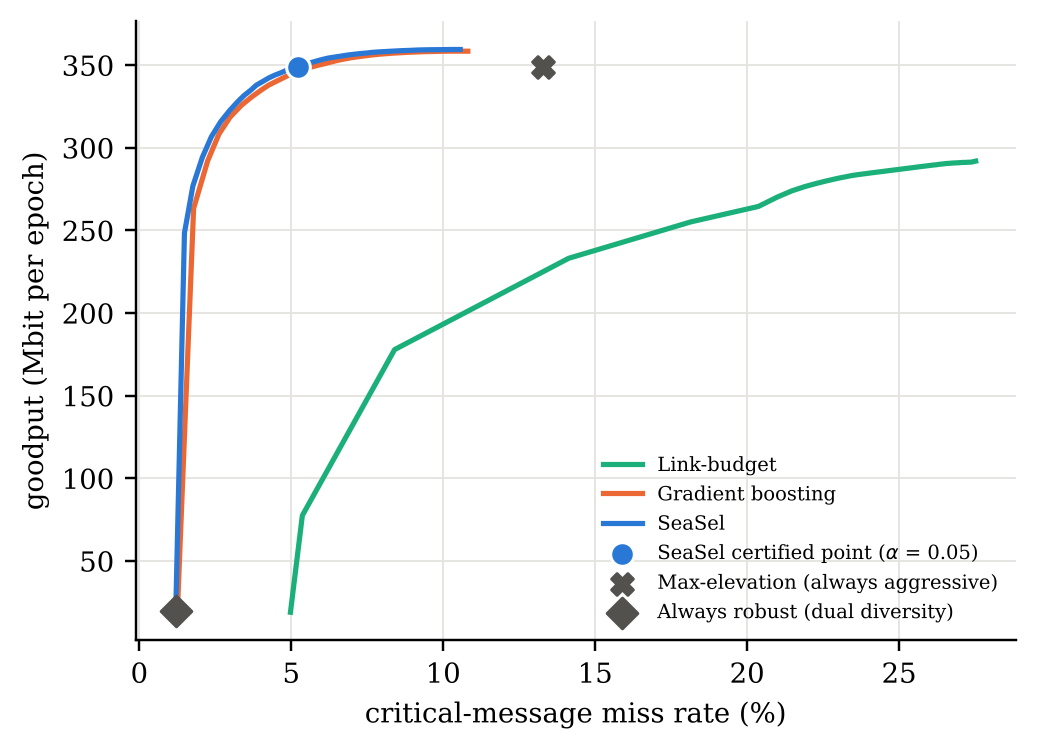
\includegraphics[width=0.62\textwidth]{../figures/fig_pareto.png}
\caption{\textbf{Goodput against critical-message miss rate.} Curves sweep the acceptance threshold; markers show the certified SeaSel operating point and the two fixed policies. SeaSel matches always-aggressive goodput while removing most of its misses.}
\label{fig:pareto}
\end{figure}

\subsection{Prediction quality and calibration}
Table~\ref{tab:disc} and Fig.~\ref{fig:riskcov} report discrimination and calibration. The SeaSel ensemble attains the highest AUROC (\RSAuroc), the lowest calibration error (\RSEce{} against \RGEce{} for gradient boosting) and the lowest area under the risk--coverage curve (\RSAurc). Its margin in AUROC over the strongest tabular baseline is small (\RSAuroc{} against \RGAuroc), so in-distribution gains in coverage are modest: SeaSel certifies \RCovGain{} percentage points more epochs than gradient boosting with the same certificate. The reliability diagram (Fig.~\ref{fig:reliability}) shows that the ensemble probabilities lie close to the diagonal, which matters because the uncertainty-penalised score (\ref{eq:choice}) uses them directly. The physics-free link-budget heuristic reaches an AUROC of only \RLAuroc, which confirms that motion, weather and history must be learned jointly.

\begin{table}[t]\centering\small
\caption{\textbf{Discrimination and calibration of the link-success predictors} on the held-out pool.}
\label{tab:disc}
\begin{tabular}{@{}lccc@{}}\toprule
Predictor & AUROC $\uparrow$ & ECE $\downarrow$ & AURC $\downarrow$\\\midrule
Link-budget margin & 0.684 & 0.209 & 0.1146\\
Logistic regression & 0.903 & 0.009 & 0.0134\\
Gradient boosting & 0.901 & 0.020 & 0.0135\\
PBA single model & 0.901 & 0.010 & 0.0136\\
SeaSel ensemble & 0.907 & 0.005 & 0.0126\\
\bottomrule\end{tabular}\end{table}

\begin{figure}[t]
\centering
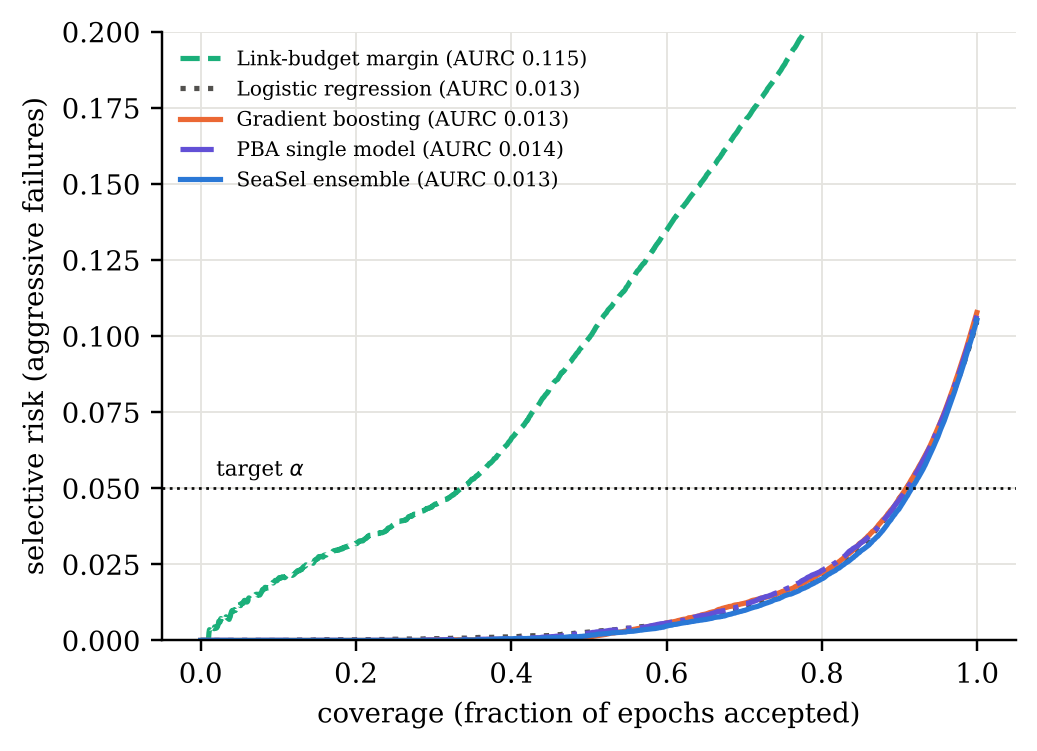
\includegraphics[width=0.6\textwidth]{../figures/fig_risk_coverage.png}
\caption{\textbf{Risk--coverage curves of the link predictors.} Selective risk of aggressive transmissions as a function of the fraction of accepted epochs.}
\label{fig:riskcov}
\end{figure}

\begin{figure}[t]
\centering
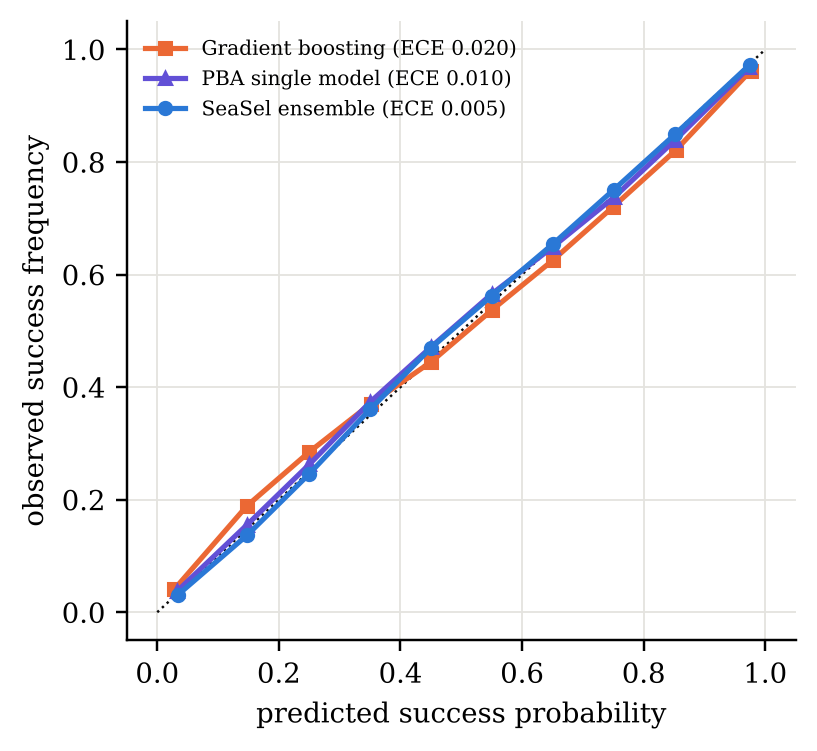
\includegraphics[width=0.5\textwidth]{../figures/fig_reliability.png}
\caption{\textbf{Reliability diagram.} Observed against predicted success probability on the evaluation pool.}
\label{fig:reliability}
\end{figure}

\subsection{Validity of the guarantee across risk targets}
Figure~\ref{fig:alpha} varies the target from $\alpha=0.02$ to $0.15$. With certification, the realised selective risk stays at or below the diagonal for every target, and the violation frequency never exceeds 0.04 for either SeaSel or certified gradient boosting. The tuned threshold lies above the diagonal for all targets up to 0.08 and violates them in every split. Certification costs coverage only where it should: at $\alpha=0.02$ SeaSel accepts 77\% of epochs, and coverage approaches 99\% at $\alpha=0.10$.

\begin{figure}[t]
\centering
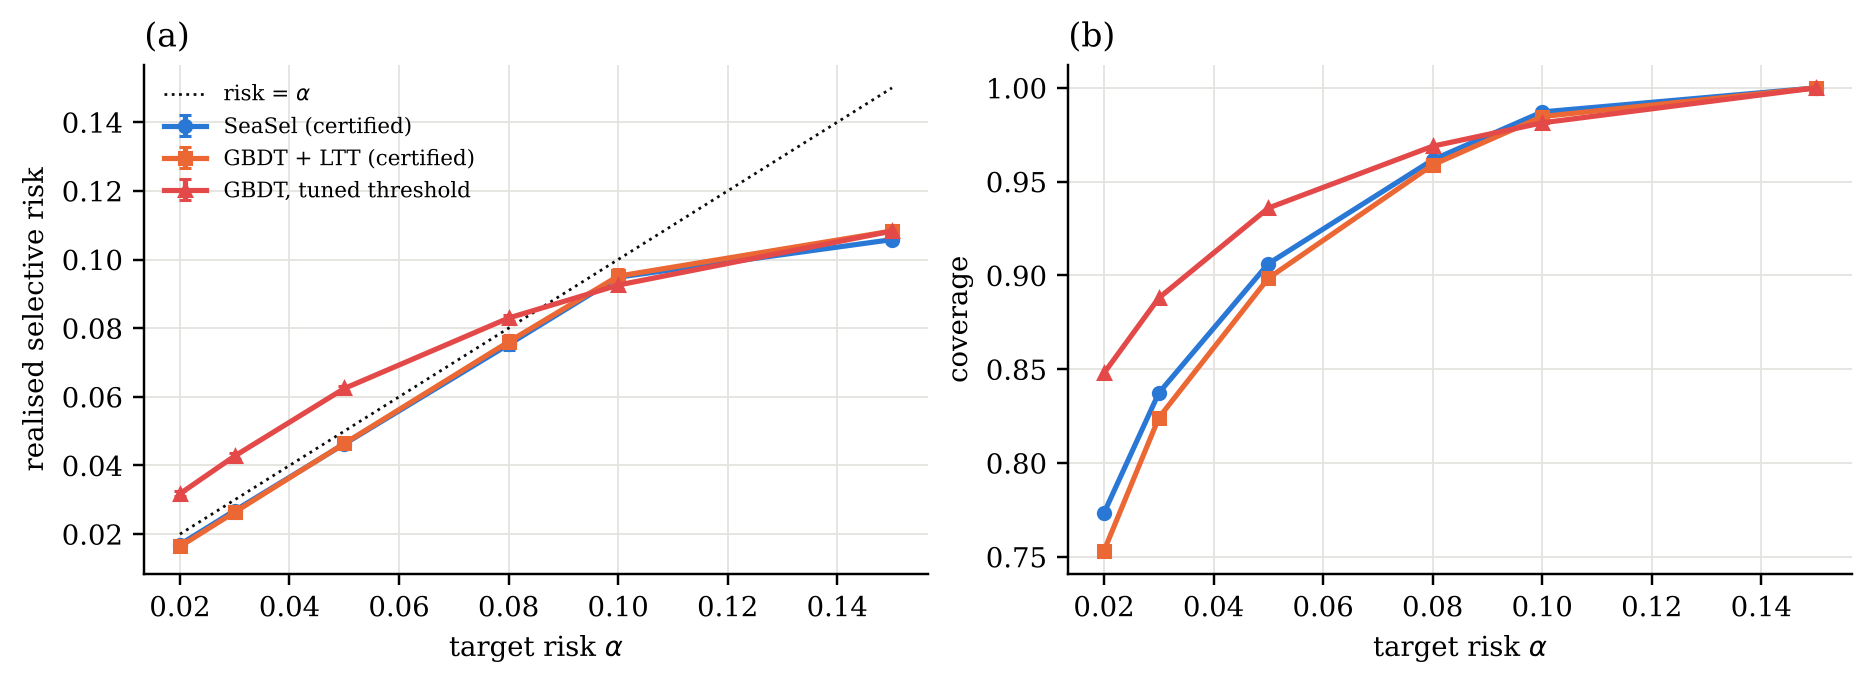
\includegraphics[width=0.95\textwidth]{../figures/fig_alpha_sweep.png}
\caption{\textbf{Guarantee validity across targets.} (\textbf{a}) Realised selective risk (mean $\pm$ s.d.\ over 60 splits) against the target $\alpha$; certified methods stay on or below the diagonal. (\textbf{b}) Coverage obtained at each target.}
\label{fig:alpha}
\end{figure}

% ===========================================================================
\section{Ablation, robustness, and OOD analyses}\label{sec:ablation}
% ===========================================================================
\subsection{Ablation}
Table~\ref{tab:ablation} removes one component at a time and retrains where necessary. The certificate keeps every variant within the target, so ablations affect only how many epochs can be accepted. Removing the link-history features (beacon deficit, blockage evidence) is by far the most damaging change: AUROC falls from \RSAuroc{} to \RAbNoHistAuroc{} and coverage from \RSCov\% to \RAbNoHistCov\%. The remaining components have small effects in distribution: removing the physics bias, replacing attention by mean pooling or by a per-link network, removing the motion context, removing the uncertainty penalty or temperature scaling, and using a single member each change coverage by less than one percentage point. In this testbed the previous beacon of each link already summarises most of the rain, blockage and motion state that the other features describe, so the per-link evidence dominates.

\begin{table}[t]\centering\small
\caption{\textbf{Ablation study} (retrained variants; $\alpha=0.05$, $\delta=0.1$, 100 splits).}
\label{tab:ablation}
\resizebox{\textwidth}{!}{\begin{tabular}{@{}lcccccc@{}}\toprule
Variant & AUROC & ECE & Coverage & Selective risk & Goodput (Mbit) & Viol.\\\midrule
\textbf{Full SeaSel} & 0.907 & 0.005 & 0.906 $\pm$ 0.002 & 0.046 $\pm$ 0.001 & 349.0 $\pm$ 0.5 & 0.01\\
Without physics bias (plain attention) & 0.906 & 0.006 & 0.905 $\pm$ 0.002 & 0.046 $\pm$ 0.001 & 348.5 $\pm$ 0.5 & 0.01\\
Mean pooling instead of attention & 0.907 & 0.007 & 0.908 $\pm$ 0.002 & 0.046 $\pm$ 0.001 & 349.6 $\pm$ 0.5 & 0.01\\
Without attention (per-link MLP) & 0.906 & 0.005 & 0.903 $\pm$ 0.002 & 0.046 $\pm$ 0.001 & 347.8 $\pm$ 0.5 & 0.01\\
Without motion and weather context & 0.906 & 0.009 & 0.906 $\pm$ 0.002 & 0.046 $\pm$ 0.002 & 349.1 $\pm$ 0.5 & 0.01\\
Without link-history features & 0.850 & 0.035 & 0.805 $\pm$ 0.005 & 0.046 $\pm$ 0.002 & 312.3 $\pm$ 1.3 & 0.02\\
Without uncertainty penalty (gamma = 0) & 0.907 & 0.005 & 0.907 $\pm$ 0.002 & 0.046 $\pm$ 0.002 & 349.2 $\pm$ 0.5 & 0.01\\
Without temperature scaling & 0.907 & 0.007 & 0.906 $\pm$ 0.002 & 0.046 $\pm$ 0.001 & 349.1 $\pm$ 0.5 & 0.01\\
Single member (M = 1) & 0.901 & 0.010 & 0.900 $\pm$ 0.002 & 0.046 $\pm$ 0.001 & 346.5 $\pm$ 0.5 & 0.02\\
\bottomrule\end{tabular}}\end{table}

\subsection{Cross-link transfer without history}
The value of reasoning across links appears when per-link evidence is missing, as for a satellite that has just risen or a terminal that has just restarted. Table~\ref{tab:transfer} retrains the three architectures with half of the satellite tokens lacking history and evaluates them in the same condition. On the tokens without history, physics-biased attention reaches an AUROC of \RTrPBAMiss, against \RTrATTMiss{} for plain attention and \RTrMLPMiss{} for the per-link network, and it certifies the largest coverage (\RTrPBACov\% against \RTrATTCov\% and \RTrMLPCov\%). The ordering is consistent but the margins are small. The geometric prior helps the model borrow evidence from nearby links, but it is a refinement of the prediction rather than the source of the guarantee.

\begin{table}[t]\centering\small
\caption{\textbf{Cross-link transfer when half of the link histories are missing} (models retrained and evaluated with 50\% of satellite tokens lacking beacon history; $\alpha=0.05$).}
\label{tab:transfer}
\resizebox{\textwidth}{!}{\begin{tabular}{@{}lcccccc@{}}\toprule
Predictor & AUROC (all) & AUROC (no history) & ECE & AURC & Coverage & Selective risk\\\midrule
Physics-biased attention & 0.881 & 0.858 & 0.015 & 0.0160 & 0.874 $\pm$ 0.003 & 0.046 $\pm$ 0.002\\
Plain attention & 0.879 & 0.854 & 0.016 & 0.0161 & 0.872 $\pm$ 0.003 & 0.046 $\pm$ 0.002\\
Per-link MLP & 0.878 & 0.850 & 0.018 & 0.0166 & 0.866 $\pm$ 0.004 & 0.046 $\pm$ 0.002\\
\bottomrule\end{tabular}}\end{table}

\subsection{Robustness to sensor corruption}
Table~\ref{tab:robust} corrupts the gateway inputs at test time. With the certificate obtained on clean data, inertial noise of 1--3$^\circ$, a threefold noisier rain gauge and 30\% missing context leave the selective risk below 5\%. Losing half of the link histories, however, raises it to 6.3\%, above the target, because the clean certificate no longer matches the input distribution. Recalibrating on data with the same corruption restores the target in every case; for missing histories this costs about four percentage points of coverage. Corruption of the history channel should therefore trigger recalibration or the online rule.

\begin{table}[t]\centering\small
\caption{\textbf{Robustness to sensor corruption at test time.} Fixed certificate from clean calibration versus recalibration on corrupted data ($\alpha=0.05$).}
\label{tab:robust}
\resizebox{\textwidth}{!}{\begin{tabular}{@{}lccccc@{}}\toprule
 & & \multicolumn{2}{c}{Clean certificate} & \multicolumn{2}{c}{Recalibrated}\\
Corruption & AUROC & Coverage & Selective risk & Coverage & Selective risk\\\midrule
IMU noise 1 deg & 0.897 & 0.918 & 0.040 & 0.931 & 0.045\\
IMU noise 3 deg & 0.875 & 0.847 & 0.027 & 0.915 & 0.045\\
Rain sensor noise x3 & 0.900 & 0.923 & 0.043 & 0.930 & 0.045\\
30\% context missing & 0.898 & 0.936 & 0.048 & 0.928 & 0.045\\
50\% link history missing & 0.874 & 0.947 & 0.063 & 0.903 & 0.045\\
\bottomrule\end{tabular}}\end{table}

\subsection{Out-of-distribution operation}
Table~\ref{tab:ood} and Fig.~\ref{fig:ood} evaluate three shifted days with the certificate obtained in distribution. Distribution shift breaks the in-distribution guarantee in all three cases: the selective risk rises to \RStormNaive\% on the severe-storm day, \RTropNaive\% on the tropical day and \RConstNaive\% when 30\% of satellites have failed. The sea-state-conditional certificate restores the target under storms (\RStormMond\%), where the shift is captured by the roll-RMS groups, but not under tropical rain or constellation loss, whose shifts are unrelated to sea state. The online rule (\ref{eq:online}) restores the target in all three cases (\RStormOnline\%, \RTropOnline\% and \RConstOnline\%) by lowering coverage to \RStormOnlineCov\%, \RTropOnlineCov\% and \RConstOnlineCov\%. Its coverage is close to that of an oracle that recalibrates on the shifted day itself. Figure~\ref{fig:ood}b shows the mechanism on the storm day: the fixed certificate lets the running risk climb to about 12\% at the height of the storm, whereas the online threshold keeps it near 5\% throughout. Always-aggressive operation would have lost \RStormAAMiss\% of critical messages on this day.

\begin{table}[t]\centering\small
\caption{\textbf{Out-of-distribution operation} (target $\alpha=0.05$). Sel.: selective risk; Cov.: coverage; Miss: critical-message miss rate.}
\label{tab:ood}
\resizebox{\textwidth}{!}{\begin{tabular}{@{}lcccccccccc@{}}\toprule
 & & \multicolumn{2}{c}{Always aggressive} & \multicolumn{2}{c}{In-distribution certificate} & \multicolumn{2}{c}{Sea-state conditional} & \multicolumn{2}{c}{Online adaptive}\\
Shift & AUROC & Sel. & Miss & Sel. & Cov. & Sel. & Cov. & Sel. & Cov.\\\midrule
Severe storms & 0.948 & 0.312 & 31.2\% & 0.057 & 0.687 & 0.048 & 0.661 & 0.049 & 0.670\\
Tropical rain & 0.906 & 0.128 & 12.8\% & 0.058 & 0.913 & 0.057 & 0.909 & 0.049 & 0.890\\
30\% satellite loss & 0.906 & 0.190 & 19.0\% & 0.101 & 0.877 & 0.101 & 0.867 & 0.050 & 0.757\\
\bottomrule\end{tabular}}\end{table}

\begin{figure}[t]
\centering
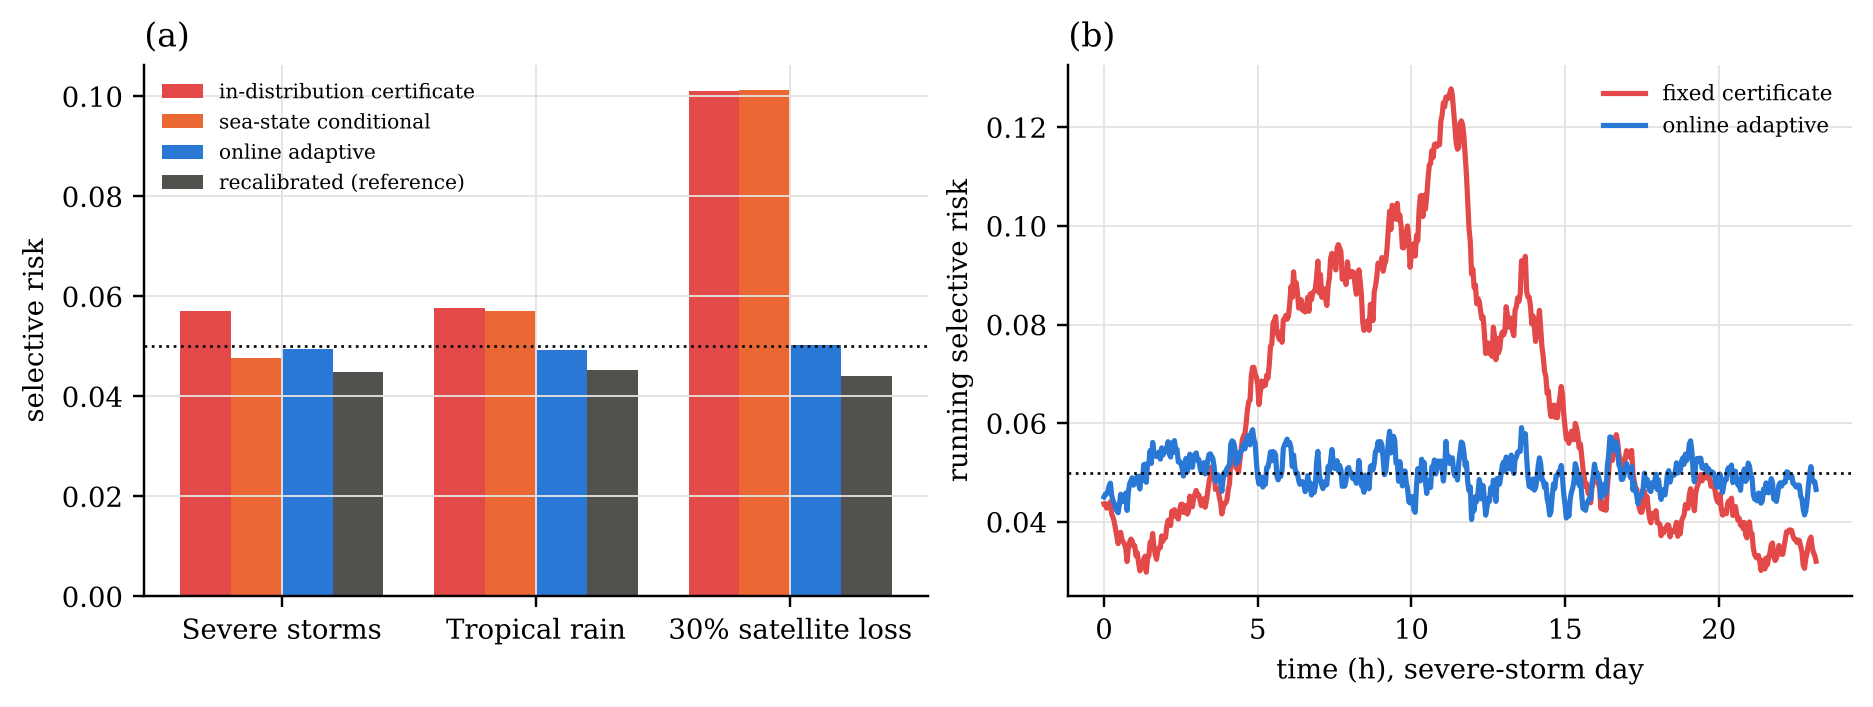
\includegraphics[width=0.95\textwidth]{../figures/fig_ood.png}
\caption{\textbf{Operation under distribution shift.} (\textbf{a}) Selective risk on three shifted days for the in-distribution certificate, the sea-state-conditional certificate, the online rule and an oracle recalibrated on the shifted day. (\textbf{b}) Running selective risk over the severe-storm day for the fixed certificate and the online rule. The dotted line marks $\alpha=0.05$.}
\label{fig:ood}
\end{figure}

% ===========================================================================
\section{Discussion, operational utility, and limitations}\label{sec:discussion}
% ===========================================================================
The results show that the main value of SeaSel lies in its decision interface rather than in its predictor. A certified threshold turns any well-calibrated link predictor into a policy with a verifiable reliability level. For a fleet operator this means alarm and safety telemetry can be given a contractual miss rate while bulk data still travel at near-aggressive rates, with no extra satellite capacity. The certificate is cheap: one calibration run per window, and \RMsDec{}\,ms per decision. The same mechanism applies to other risk-sensitive decisions on a vessel gateway, such as choosing a modulation order, scheduling handovers or deciding when to store and forward. Three limitations remain. First, all results come from a simulated testbed; field logs from vessels are needed to confirm the channel and motion models, although the certificate itself remains valid for any data that satisfy its exchangeability assumption. Second, the guarantee holds only under exchangeability, so drift must be handled by recalibration or by the online rule, whose guarantee is asymptotic. Third, the architectural gains of physics-biased attention are modest in distribution; larger fleets, richer beam-level telemetry and three-dimensional ray geometry may increase them.

% ===========================================================================
\section{Conclusion}\label{sec:conclusion}
% ===========================================================================
This paper introduced SeaSel, a framework that lets a vessel gateway act on learned satellite-link predictions only when a finite-sample certificate guarantees that accepted decisions rarely fail. The framework combines a physics-biased attention ensemble over all candidate links, a Learn-then-Test certificate with exact binomial p-values, a dual-link robust fallback with an explicit service-level bound, and sea-state-conditional and online variants for distribution shift. On a sandbox testbed with a two-shell constellation, storms, ship motion and blockage, SeaSel held the selective risk at \RSRisk\% for a 5\% target and cut critical-message misses by \RMissRed\% without losing goodput. Uncertified thresholds violated the target in almost every split. Under storms, tropical rain and constellation degradation, the online rule restored the target where the fixed certificate failed. The results also show where the gains come from: link history is the most informative input, calibration quality determines how many epochs can be certified, and drift is the main threat to the guarantee. Future work will validate the framework on field logs from vessels, extend it to multi-vessel coordination and inter-satellite routing, and study certificates that adapt to sea state, season and constellation health together.


\section*{Data availability}
All data analysed in this study were generated with the open sandbox testbed described in Section~\ref{sec:setup}. The generated datasets and raw results are available in the code repository listed below.

\section*{Code availability}
The complete implementation (testbed, models, certification, experiments, figures and manuscript sources) is available at \texttt{https://github.com/<account>/seasel-maritime-satellite-iot} (to be made public on submission).

\section*{Acknowledgements}
The author thanks St. Xavier's Catholic College of Engineering, Nagercoil, for institutional support.

\section*{Author contributions}
A.B.V.L. conceived the study, developed the framework and algorithm, implemented the testbed and experiments, analysed the results and wrote the manuscript.

\section*{Funding}
This research received no specific grant from any funding agency in the public, commercial or not-for-profit sectors.

\section*{Competing interests}
The author declares no competing interests.

\section*{Additional information}
\textbf{Correspondence} and requests for materials should be addressed to A.B.V.L. (bamilavirgin@sxcce.edu.in).

\begin{thebibliography}{99}
\small
\bibitem{xia2020} Xia, T., Wang, M. M., Zhang, J. \& Wang, L. Maritime Internet of Things: Challenges and Solutions. \emph{IEEE Wireless Commun.} \textbf{27}, 188--196 (2020). https://doi.org/10.1109/mwc.001.1900322
\bibitem{alqurashi2023} Alqurashi, F. S., Trichili, A., Saeed, N., Ooi, B. S. \& Alouini, M.-S. Maritime Communications: A Survey on Enabling Technologies, Opportunities, and Challenges. \emph{IEEE Internet Things J.} \textbf{10}, 3525--3547 (2023). https://doi.org/10.1109/jiot.2022.3219674
\bibitem{shang2025} Shang, Z., Zhang, X. \& Li, X. Maritime communication networks: A survey on architecture, key technologies, and challenges. \emph{Comput. Commun.} \textbf{241}, 108255 (2025). https://doi.org/10.1016/j.comcom.2025.108255
\bibitem{chen2021ch} Chen, W., Li, C., Yu, J., Zhang, J. \& Chang, F. A survey of maritime communications: From the wireless channel measurements and modeling perspective. \emph{Reg. Stud. Mar. Sci.} \textbf{48}, 102031 (2021). https://doi.org/10.1016/j.rsma.2021.102031
\bibitem{nomikos2024} Nomikos, N. \emph{et al.} Improving Connectivity in 6G Maritime Communication Networks With UAV Swarms. \emph{IEEE Access} \textbf{12}, 18739--18751 (2024). https://doi.org/10.1109/access.2024.3360133
\bibitem{kodheli2021} Kodheli, O. \emph{et al.} Satellite Communications in the New Space Era: A Survey and Future Challenges. \emph{IEEE Commun. Surv. Tutor.} \textbf{23}, 70--109 (2021). https://doi.org/10.1109/comst.2020.3028247
\bibitem{michel2022} Michel, F., Trevisan, M., Giordano, D. \& Bonaventure, O. A first look at starlink performance. In \emph{Proceedings of the 22nd ACM Internet Measurement Conference} 130--136 (ACM, 2022). https://doi.org/10.1145/3517745.3561416
\bibitem{laniewski2024} Laniewski, D. \emph{et al.} Starlink on the Road: A First Look at Mobile Starlink Performance in Central Europe. In \emph{2024 8th Network Traffic Measurement and Analysis Conference (TMA)} 1--8 (IEEE, 2024). https://doi.org/10.23919/tma62044.2024.10559110
\bibitem{lin2021} Lin, X., Rommer, S., Euler, S., Yavuz, E. A. \& Karlsson, R. S. 5G from Space: An Overview of 3GPP Non-Terrestrial Networks. \emph{IEEE Comm. Stand. Mag.} \textbf{5}, 147--153 (2021). https://doi.org/10.1109/mcomstd.011.2100038
\bibitem{liu2018} Liu, J., Shi, Y., Fadlullah, Z. M. \& Kato, N. Space-Air-Ground Integrated Network: A Survey. \emph{IEEE Commun. Surv. Tutor.} \textbf{20}, 2714--2741 (2018). https://doi.org/10.1109/comst.2018.2841996
\bibitem{guo2022} Guo, H., Li, J., Liu, J., Tian, N. \& Kato, N. A Survey on Space-Air-Ground-Sea Integrated Network Security in 6G. \emph{IEEE Commun. Surv. Tutor.} \textbf{24}, 53--87 (2022). https://doi.org/10.1109/comst.2021.3131332
\bibitem{hu2026} Hu, X., Lin, B., Wang, P. \& Lu, X. LEO Satellite and UAV-Assisted Maritime Internet of Things: Modeling and Performance Analysis for Data Acquisition. \emph{Future Internet} \textbf{18}, 24 (2026). https://doi.org/10.3390/fi18010024
\bibitem{wu2019} Wu, Y., Hu, G., Jin, F. \& Zu, J. A Satellite Handover Strategy Based on the Potential Game in LEO Satellite Networks. \emph{IEEE Access} \textbf{7}, 133641--133652 (2019). https://doi.org/10.1109/access.2019.2941217
\bibitem{chen2024ho} Chen, J., Ozger, M. \& Cavdar, C. Nash Soft Actor-Critic LEO Satellite Handover Management Algorithm for Flying Vehicles. In \emph{2024 IEEE International Conference on Machine Learning for Communication and Networking (ICMLCN)} 380--385 (IEEE, 2024). https://doi.org/10.1109/icmlcn59089.2024.10624798
\bibitem{chen2026sr} Chen, J., Jiang, H. \& Chu, R. Graph-guided MADQN based handover strategy for LEO satellite networks. \emph{Sci. Rep.} \textbf{16}, 35970 (2026). https://doi.org/10.1038/s41598-026-69734-6
\bibitem{pan2020} Pan, M., Hu, J., Yuan, J., Liu, J. \& Su, Y. An Efficient Blind Doppler Shift Estimation and Compensation Method for LEO Satellite Communications. In \emph{2020 IEEE 20th International Conference on Communication Technology (ICCT)} 643--648 (IEEE, 2020). https://doi.org/10.1109/icct50939.2020.9295821
\bibitem{zhu2022} Zhu, Y., Hofmann, C. A. \& Knopp, A. Ka-Band LEO Satellite Internet of Things Channel Characterization: Survey and Measurement. In \emph{ICC 2022 - IEEE International Conference on Communications} 3076--3081 (IEEE, 2022). https://doi.org/10.1109/icc45855.2022.9838878
\bibitem{weerackody2006} Weerackody, V. \& Gonzalez, L. Motion Induced Antenna Pointing Errors in Satellite Communications On-The-Move Systems. In \emph{2006 40th Annual Conference on Information Sciences and Systems} 961--966 (IEEE, 2006). https://doi.org/10.1109/ciss.2006.286605
\bibitem{gomez2018} Gómez, I. \emph{et al.} Field trials of the VHF data exchange system (VDES) satellite downlink component. In \emph{36th International Satellite Communications Systems Conference (ICSSC2018)} 25 (Institution of Engineering and Technology, 2018). https://doi.org/10.1049/cp.2018.1706
\bibitem{chow1970} Chow, C. On optimum recognition error and reject tradeoff. \emph{IEEE Trans. Inform. Theory} \textbf{16}, 41--46 (1970). https://doi.org/10.1109/tit.1970.1054406
\bibitem{hendrickx2024} Hendrickx, K., Perini, L., Van der Plas, D., Meert, W. \& Davis, J. Machine learning with a reject option: a survey. \emph{Mach. Learn.} \textbf{113}, 3073--3110 (2024). https://doi.org/10.1007/s10994-024-06534-x
\bibitem{vovk2022} Vovk, V., Gammerman, A. \& Shafer, G. \emph{Algorithmic Learning in a Random World} 2nd edn (Springer International Publishing, 2022). https://doi.org/10.1007/978-3-031-06649-8
\bibitem{angelopoulos2023} Angelopoulos, A. N. \& Bates, S. Conformal Prediction: A Gentle Introduction. \emph{Found. Trends Mach. Learn.} \textbf{16}, 494--591 (2023). https://doi.org/10.1561/2200000101
\bibitem{bates2021} Bates, S., Angelopoulos, A., Lei, L., Malik, J. \& Jordan, M. Distribution-free, Risk-controlling Prediction Sets. \emph{J. ACM} \textbf{68}, 1--34 (2021). https://doi.org/10.1145/3478535
\bibitem{angelopoulos2025} Angelopoulos, A. N., Bates, S., Candès, E. J., Jordan, M. I. \& Lei, L. Learn then test: Calibrating predictive algorithms to achieve risk control. \emph{Ann. Appl. Stat.} \textbf{19}, 1641--1662 (2025). https://doi.org/10.1214/24-aoas1998
\bibitem{cohen2023} Cohen, K. M., Park, S., Simeone, O. \& Shamai Shitz, S. Calibrating AI Models for Wireless Communications via Conformal Prediction. \emph{IEEE Trans. Mach. Learn. Commun. Netw.} \textbf{1}, 296--312 (2023). https://doi.org/10.1109/tmlcn.2023.3319282
\bibitem{brauwers2023} Brauwers, G. \& Frasincar, F. A General Survey on Attention Mechanisms in Deep Learning. \emph{IEEE Trans. Knowl. Data Eng.} \textbf{35}, 3279--3298 (2023). https://doi.org/10.1109/tkde.2021.3126456
\bibitem{abdar2021} Abdar, M. \emph{et al.} A review of uncertainty quantification in deep learning: Techniques, applications and challenges. \emph{Inf. Fusion} \textbf{76}, 243--297 (2021). https://doi.org/10.1016/j.inffus.2021.05.008
\bibitem{barber2023} Barber, R. F., Candès, E. J., Ramdas, A. \& Tibshirani, R. J. Conformal prediction beyond exchangeability. \emph{Ann. Statist.} \textbf{51}, 816--845 (2023). https://doi.org/10.1214/23-aos2276
\bibitem{hoeffding1963} Hoeffding, W. Probability Inequalities for Sums of Bounded Random Variables. \emph{J. Am. Stat. Assoc.} \textbf{58}, 13--30 (1963). https://doi.org/10.1080/01621459.1963.10500830
\end{thebibliography}


\end{document}
